\pagestyle{fancy}
\fancyhf{}
\renewcommand{\headrulewidth}{0pt}
\fancyfoot[C]{\leftmark}
\fancyhead[R]{\thepage}
\doublespacing
\chapter{Response of a glassy system to thermal gradient}\label{chap3}

\noindent\fbox{\parbox{\textwidth}
    {\color{myred}
    This chapter is based on the following publication \cite{vaibhav2020response}:\\
    {\em Response of glassy liquids to thermal gradients}\\
    V. Vaibhav, J. Horbach, and P. Chaudhuri, Phys. Rev. E 101, 022605 (2020)}
}

\section{Introduction} 

Many glass-forming liquids are intrinsically polydisperse or multi-component in their constituent properties \cite{glassbook}, via which crystallization is kinetically suppressed and thus glasses are formed.  Multi-component glasses, in various form, are ubiquitous in diverse applications or natural phenomena and in many such cases, the non-equilibrium response of such systems to external stimuli, e.g.~heat or mechanical load, is of significance. However, from a microscopic perspective, the response to externally imposed temperature gradients, especially even of binary glass-forming liquids, is not well understood. Here, in this chapter, we focus on this issue using non-equilibrium molecular dynamics simulations.

As we have also discussed in Chapter-\ref{chap2}, when a temperature gradient is applied to any mixture, there is a resultant flux of matter. This is known as the Ludwig-Soret effect \cite{ludwig,soret,degroot}, which has been extensively studied \cite{ikeshoji1994, reith, artola07, platten2006, bresme2014, koehler2016, ciccotti2017} in fluid mixtures under ``normal conditions'', i.e.~far away from the glass transition.  In the linear response regime, for a binary mixture with an asymmetry, e.g., in size, charge, mass or interaction energy, this effect is characterized by the Soret coefficient, defined as $S_T=D_T/D_{AB}$ with $D_{AB}$ the interdiffusion coefficient and $D_T$ the thermal diffusion coefficient (also check Chapter-\ref{chap2} for further details). While $D_T$ is a measure of the cross-correlations between thermal and mass fluxes, $D_{AB}$ is associated with the mass transport induced by concentration gradients. Thus, $S_T$ measures the relative strength of the latter processes.

\section{Objective}

For glassy materials, inhomogeneous thermal conditions are encountered under diverse circumstances, e.g.~during the formation of the glass from the supercooled melt via cooling \cite{angell1986, liu, clever2012, ediger2017}, densification \cite{rauch2002}, or in cases where the material is heated non-uniformly \cite{physicslava, lacks, liu11}.  During the glass formation, there is a fundamental difference between the transport of heat and processes such as interdiffusion which are associated with the mass transport.  Structural relaxation becomes increasingly slow as the glass transition is approached, and, as a consequence, a drastic slowing down and eventually a dynamical arrest of the interdiffusive transport takes place. The heat flux, however, remains a fast process in the supercooled liquid and even in the glass state \cite{mizuno,bhuyan,gotze89,scheidler01}.

%%%%%%%%%
Our objective is to investigate the coupling between thermal diffusion and interdiffusion processes, as the ambient temperatures are varied from the supercooled to the glassy regime. In the vicinity of the glass transition, one may expect a strong nonlinear coupling of the two transport processes as well as long-lived non-stationary structures, at least in regions where the local temperature is below the glass transition temperature, which we analyse.

%Using extensive molecular dynamics (MD) simulations, we investigate the response of a model glass-forming liquid to an applied thermal gradient. We show that with decreasing temperature the concentration gradients increase and the nonlinear response sets in at smaller thermal gradients. However, in the glass state, the prohibitively slow dynamics suppresses the onset of such concentration inhomogeneities in response to the thermal gradient. Here, local melting in zones above the glass transition temperature leads to various anomalies, including history-dependent responses. Below, we show that our observations are due to the negative mixing enthalpy of the considered glass-forming mixture as well as the decoupling in the dynamical behaviour of the constituent species.

%The paper is organised in the following way. In section II, we describe the details of the model glass former that is used for the MD simulations, as well as the numerical method used for probing the non-equilibrium response of the system. In section III, we discuss the findings of our study, and then we provide a concluding discussion in section IV.

\section{Model and method}

For our study, we consider the well-studied glass-forming Kob-Andersen 80:20 binary AB Lennard-Jones (LJ) mixture,  originally proposed to model amorphous $Ni_{80}P_{20}$ \cite{Kob94}. The details related to this model glass former are in section-\ref{model} of Chapter-\ref{chap2}.  

Following Ref.\cite{Kob94}, we have chosen $\epsilon_{\rm{AA}} = 1.0$, $\epsilon_{\rm{AB}} = 1.5\epsilon_{\rm{AA}}$; $\epsilon_{\rm{BB}} = 0.5\epsilon_{\rm{AA}}$ for the parameters with unit of energy and $\sigma_{\rm{AA}} = 1.0$, $\sigma_{\rm{AB}} = 0.8\sigma_{\rm{AA}}$, $\sigma_{\rm{BB}} = 0.88\sigma_{\rm{AA}}$ for those with unit of length. The range of the interactions is set to $R_{c} = 2.5\sigma_{\rm{AA}}$. All particles have the same mass $m=1$.  All measured quantities are expressed in LJ units, whereby lengths and energies are expressed in units of $\sigma_{\rm AA}$ and $\varepsilon_{\rm AA}$, respectively.  The unit of time is $\sqrt{{m\sigma_{\rm
AA}^{2}}/\varepsilon_{\rm AA}}$.

For this model, the mode-coupling temperature, below which equilibrium dynamics is difficult to observe, occurs around $T_{\rm MCT}=0.435$ and the glass transition is estimated at $T_{\rm VFT}\approx{0.3}$.  Note that the majority A species and the minority B species have a size asymmetry $\sigma_{AA}/\sigma_{BB}\approx1.14$ and the choice of the energy parameters in the LJ model,  $\varepsilon_{\rm AB}/\varepsilon_{\rm AA}=1.5$ and  $\varepsilon_{\rm AB}/\varepsilon_{\rm BB}=3.0$, provides  a negative mixing enthalpy and a strong stability against fluid-fluid demixing \cite{toxvaerd09,pedersen18,amore11}.

In our work, we consider a system of $N=22500$ particles in a rectangular box of dimension $L_x = L_y = 14.12$ and $L_z = 94.10$, with periodic boundary conditions. The MD simulations are carried out by numerically integrating the equations of motion of the $N$ particles via the velocity Verlet algorithm, with a time step of $\delta{t}=0.005$, using LAMMPS \cite{lammps}.

Both in the equilibrium and non-equilibrium simulations, respective global and local temperatures are maintained via Langevin thermostat (see section\ref{thermostat} in Chapter-\ref{chap2}), using a dissipation timescale of $\tau_d=0.5$. At temperatures where this model system behaves as an equilibrium liquid, we first equilibrate it by coupling it to the thermostat to maintain the desired temperature $T_m$. To study the response to a thermal gradient, we locally thermostat a region of width $L_z/10$ in the middle at lower temperature $T_{\rm c}$ [marked ``Cold'' in the schematic diagram, Fig.~\ref{fig3p1}(a)] and another two regions of width $L_z/20$ at the two extreme ends at higher temperature $T_{\rm h}$ [marked ``Hot'' in Fig.~\ref{fig3p1}(a)] \cite{ikeshoji1994}. $T_{\rm h}$ and $T_{\rm c}$ are chosen symmetrically about the mean temperature $T_m$. The intermediate regions adapt to these thermal baths, and we thereby study the response to the applied gradient.

All measurements are averaged over 30-65 independent trajectories, by separately quenching high temperature liquid ($T=3.0$) states to different target temperatures ($T_m$) in the supercooled regime, followed by a sufficiently long run to reach equilibrium, in respective trajectories, at that temperature. The well-equilibrated configurations are prepared for the following temperatures: $1.0, 0.9, 0.8, 0.7, 0.6, 0.55, 0.5$, and their number varies, e.g. $65$ for $T_m = 0.5$, $30$ for $T_m = 1.0$.  Similarly, around 65 independent glassy states at $T_m=0.2$ are prepared by quenching high-temperature liquid states to this temperature, and then each configuration is aged for a period of $t_{\rm age} = 10^4$.

In the non-equilibrium simulations, after imposing the temperature gradient to the prepared states, spatial profiles of different quantities like heat flux, concentration, density etc.~are  measured using 80 bins along $L_z$. In the supercooled regime, measurements are done when the system reaches the steady state (as described below), while measurements for glassy states are done during the transient regime, since steady state in terms of spatial variation of concentration is not reached. The total length of runs, after switching on the gradient, has been done for $6 \times 10^8$ timesteps for lower temperature like $T_m = 0.5$ and $3 \times 10^8$ timesteps for higher temperatures like $T_m = 1.0$. In the case of $T_m=0.2$, the glass samples have been exposed to thermal gradient for $1 \times 10^8$ timesteps.

\begin{figure}[hbt!]
    \centering
	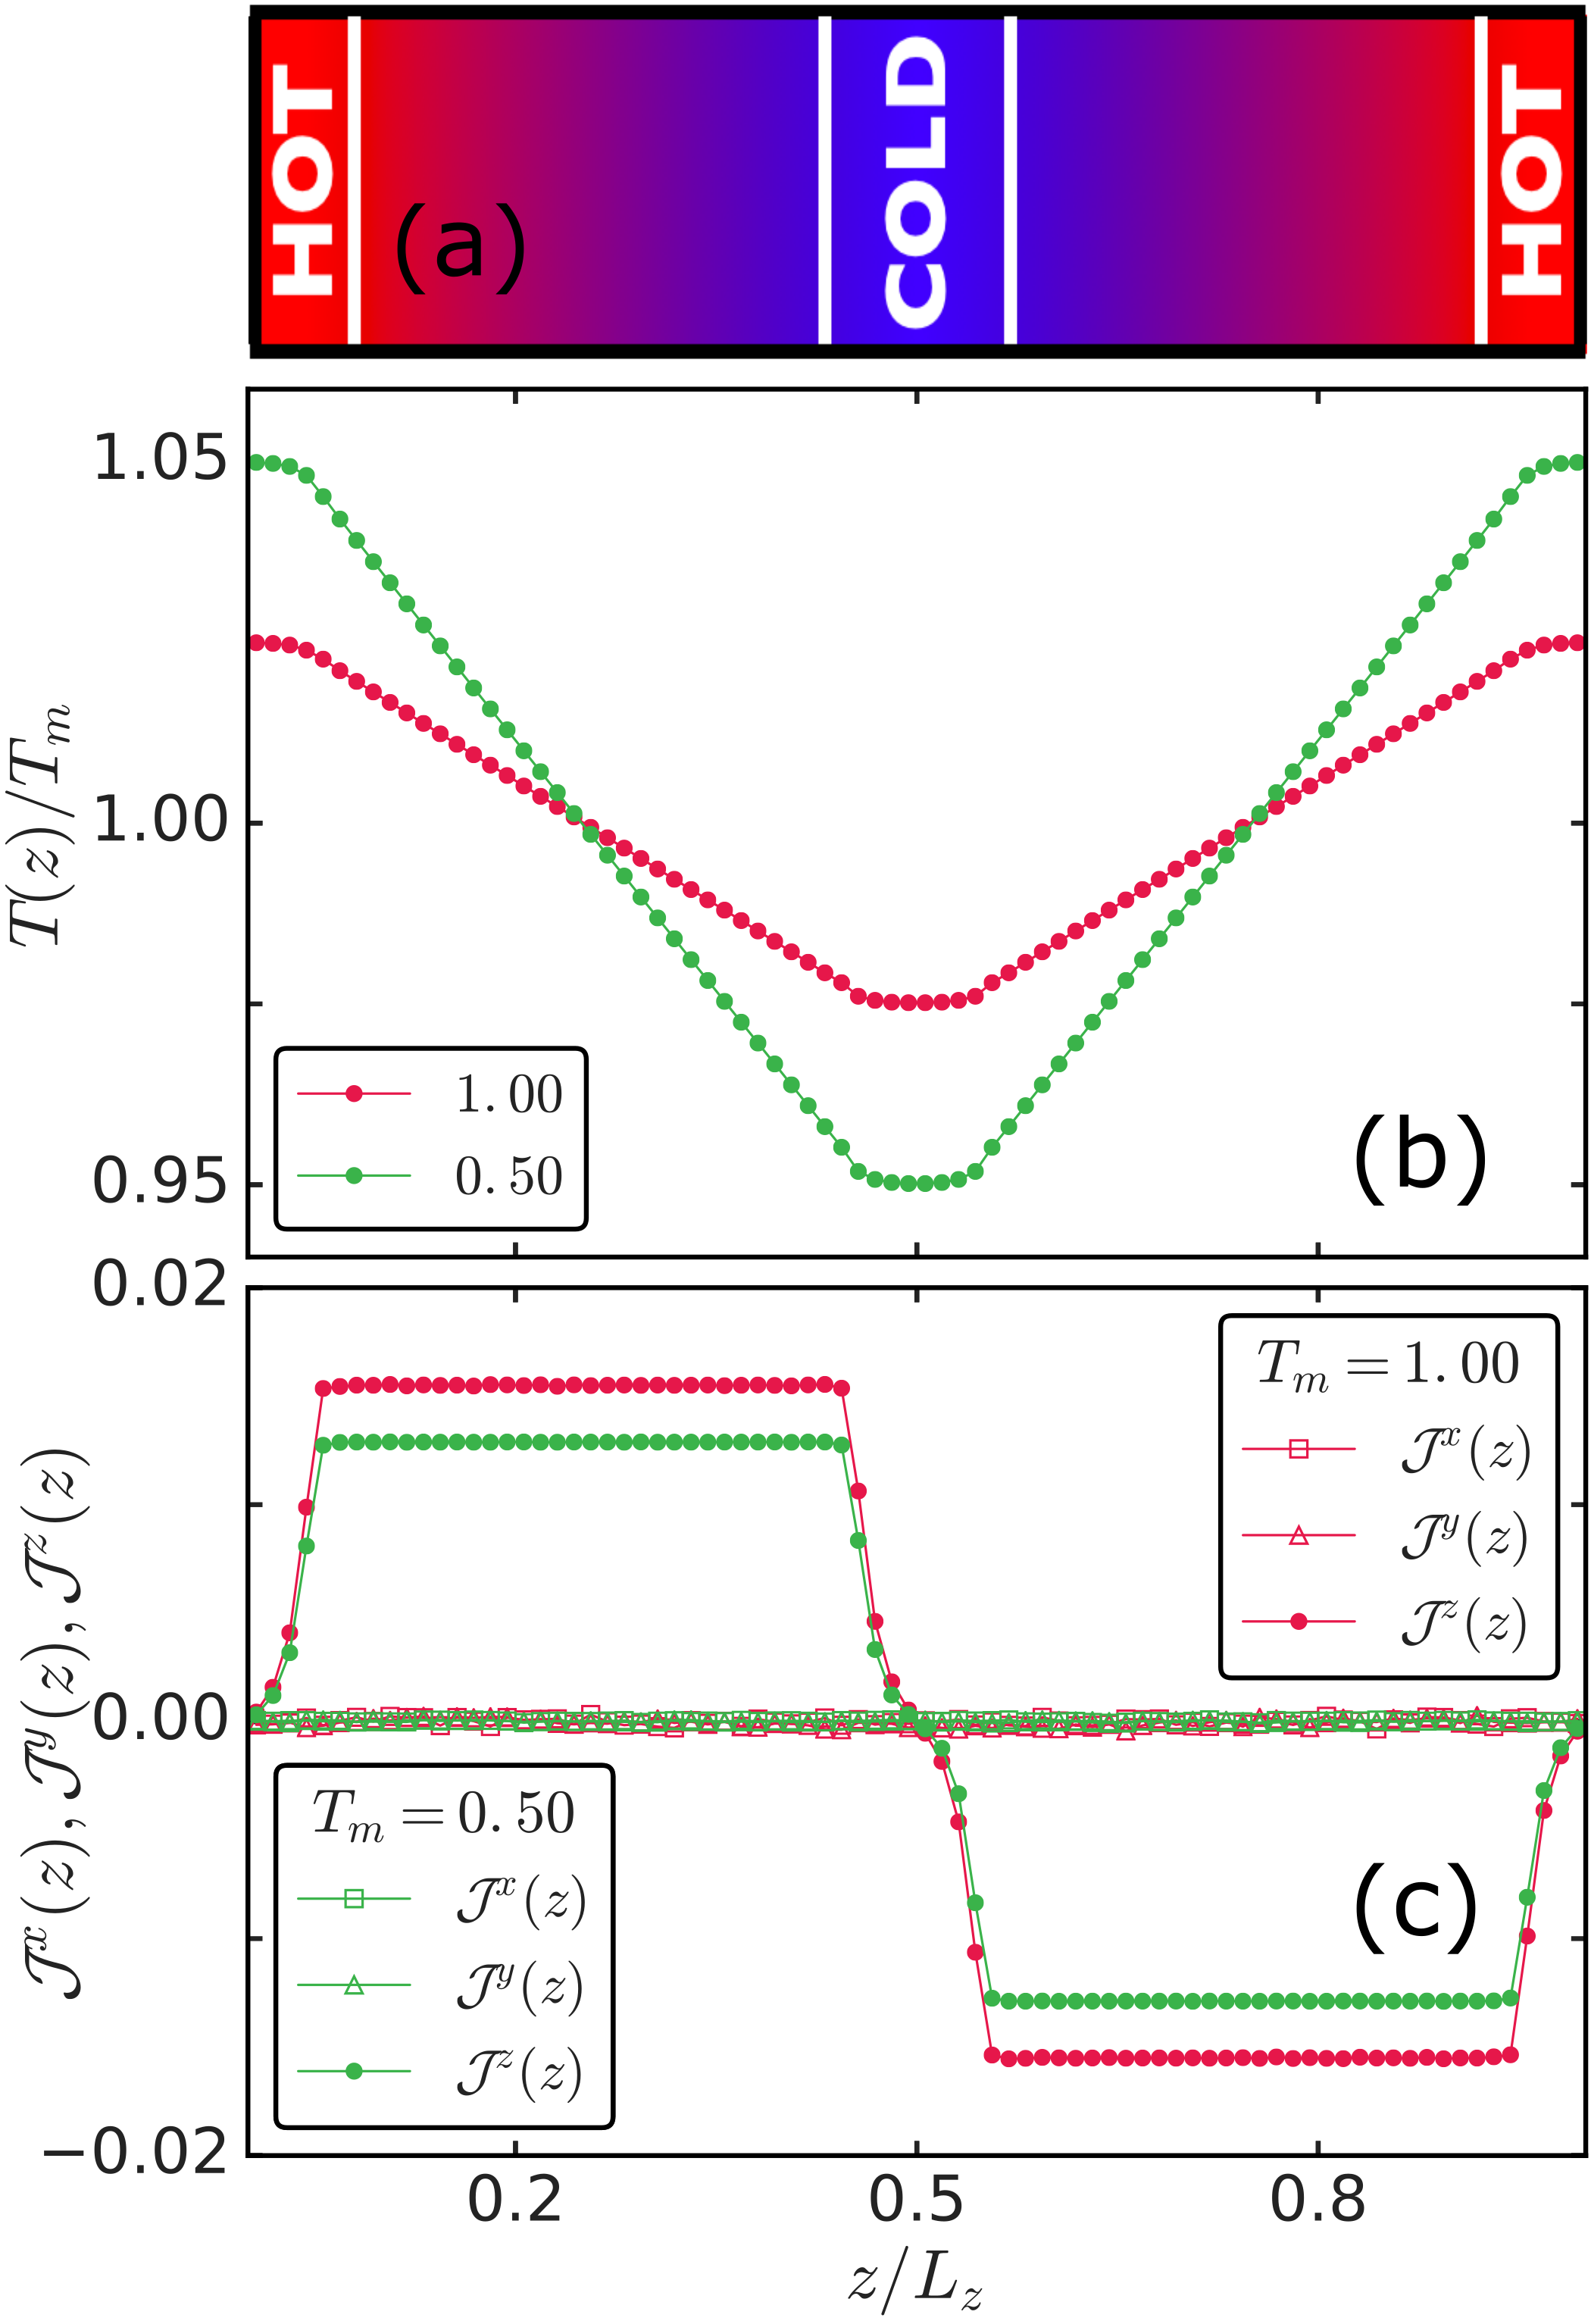
\includegraphics[width=12cm]{figs/fig3p1.png}	
	\caption[{\em Schematic of the sumulation set-up, applied temperature gradient and resulting heat current}]{(a) Schematic of the simulation set-up.
		(b) Typical spatial profile of temperature along $z$ direction, shown for $T_m=1.0, 0.5$. 
		(c) Corresponding spatial profiles
		of the heat current along the $x, y, z$ direction.  \label{fig3p1}}
\end{figure}

\begin{figure}[hbt!]
    \centering
	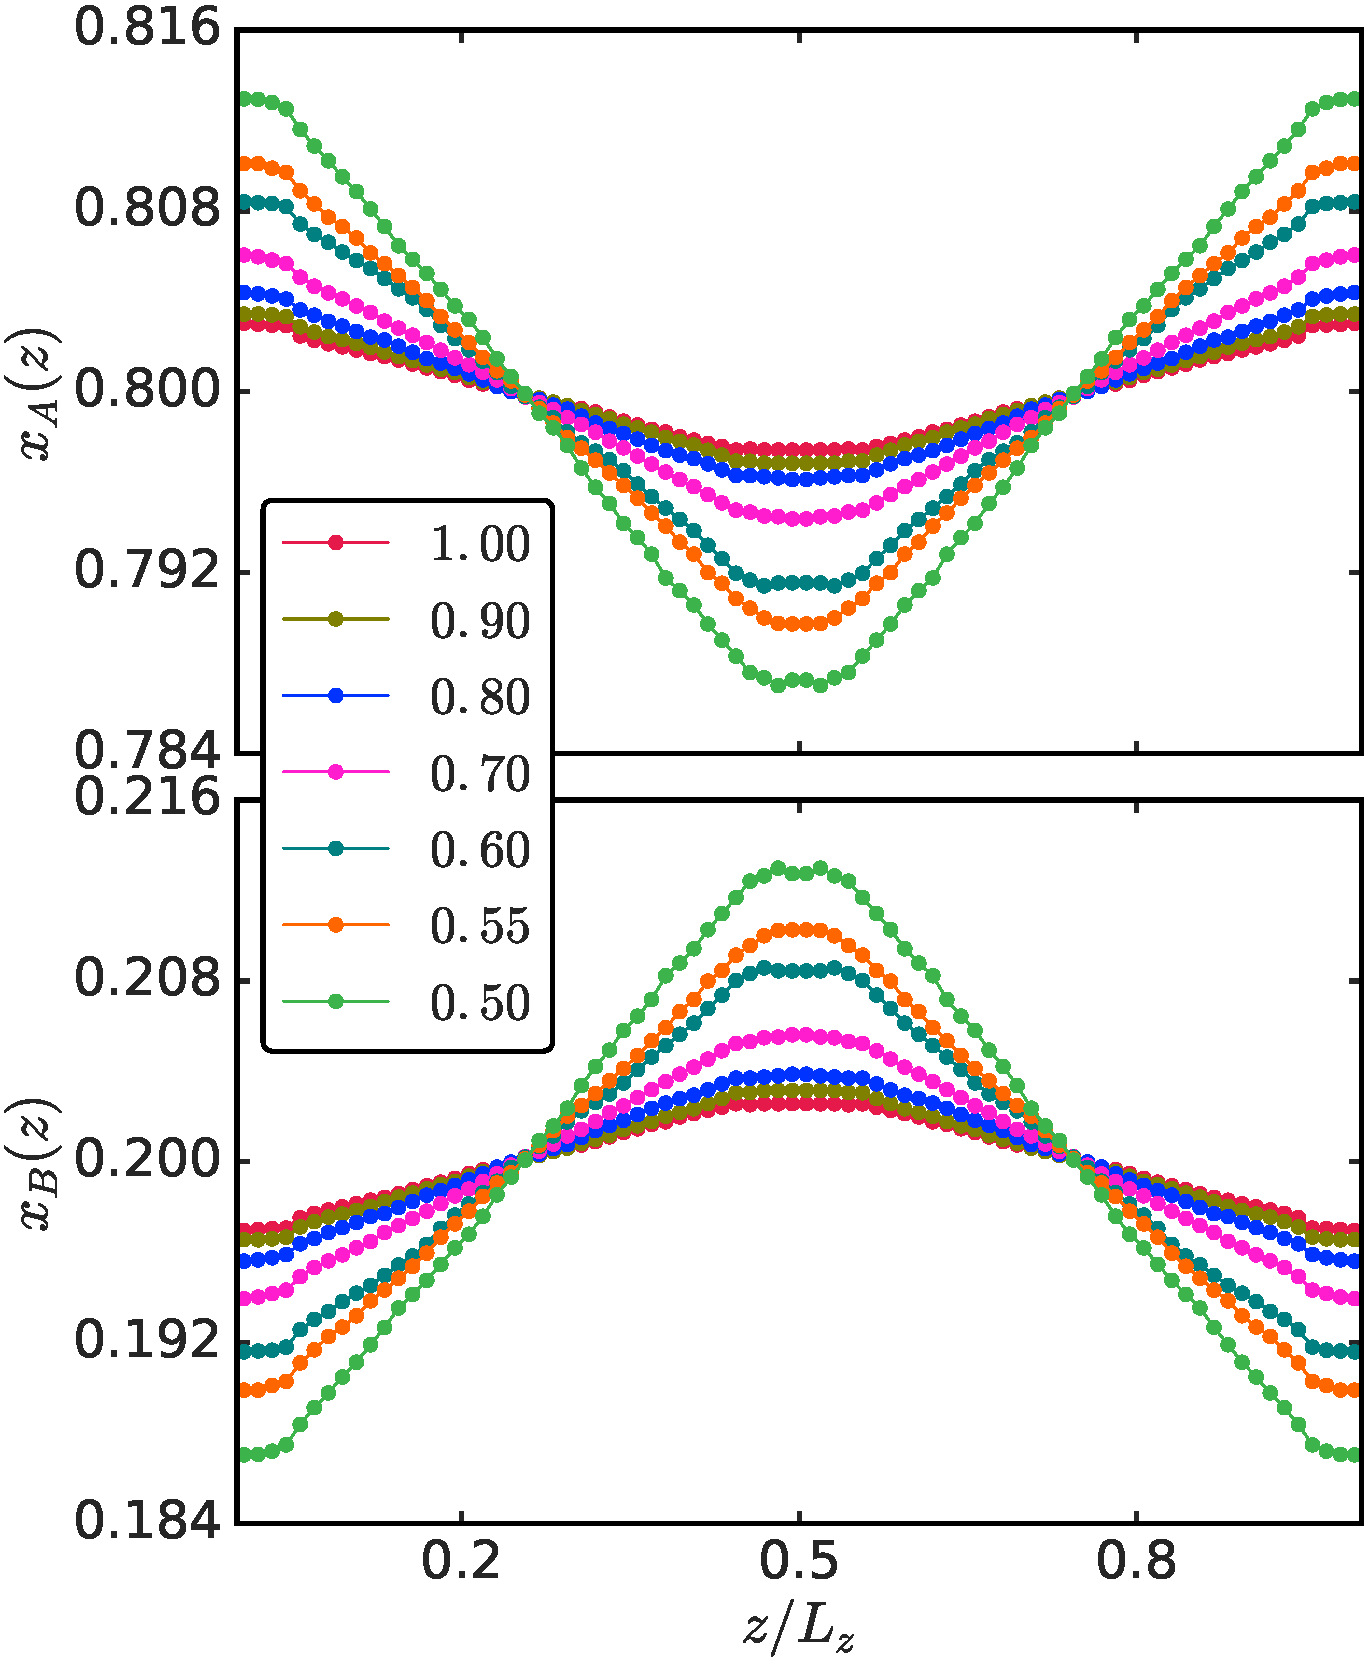
\includegraphics[width=11cm]{figs/fig3p2top.pdf}
	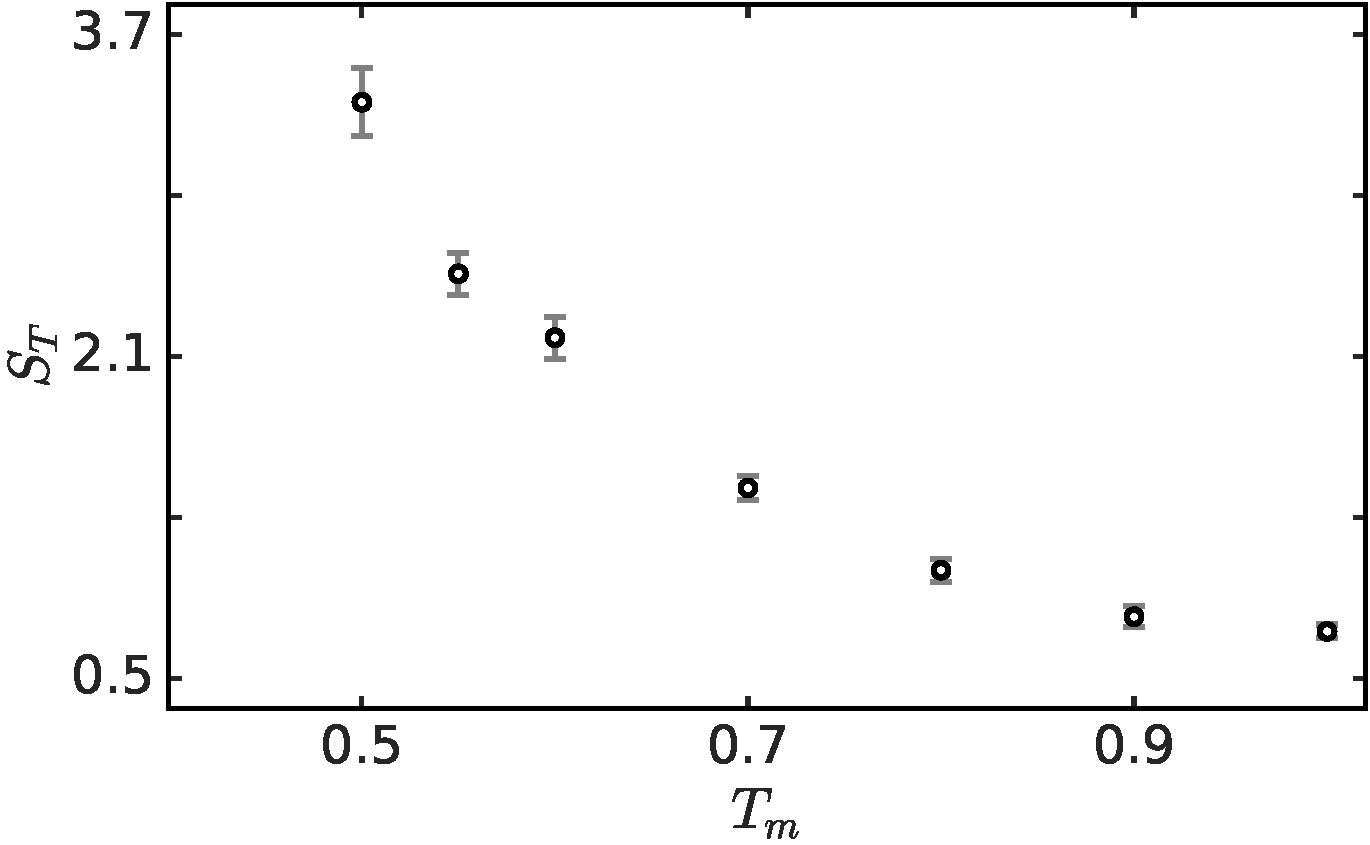
\includegraphics[width=11cm]{figs/fig3p2bottom.pdf}
	\caption[{\em Concentration profiles and Soret coefficeint measured as a function of mean temperature}]{(Top) Spatial concentration profiles of A and B particles for $T_m=1.00$, 0.90, 0.80, 0.70, 0.60, 0.55, 0.50. (Bottom) Corresponding Soret coefficient (absolute value).\label{fig3p2}}
\end{figure}


%%

\section{Results}

\subsection{Response in the supercooled regime} 

We first consider the case where the mean temperature $T_m$ resides at temperatures in the supercooled liquid regime.  Fig.~\ref{fig3p1}(b) shows examples of the linear temperature profiles that are set up, keeping $T_{\rm h}=T_m+0.5\Delta{T}$ and $T_{\rm c}=T_m-0.5\Delta{T}$ between the hot and cold ends, respectively.  Correspondingly, there is a finite heat current, $J^z(z)$, that develops in $z$ direction, and no currents in the orthogonal directions, as is shown in Fig.~\ref{fig3p1}(c). The measurement of heat current density in a bin is done via the following expression: 
%\begin{eqnarray}
%\label{heatFlux}
$J^{\alpha} = \sum_l J^{\alpha}_l = \frac{1}{V} \sum_{l} \Big[ \sum_{\beta \in \{x, y, z\}} (e_l \delta_{\alpha \beta}  - S^{\alpha \beta}_l)v^{\beta}_l \Big]$,
%\end{eqnarray}
where $J^{\alpha}$ is one of the components of the heat current density, $l$ is summed over the number of particles in the bin with volume $V$,  and $e_l$, $v^{\beta}_l$ and  $S^{\alpha \beta}_l$  are the total energy (here, the sum of kinetic and potential energy), component of the velocity  and component of the stress tensor associated with the $l${th} particle in the bin, respectively.

As expected in the steady state, the heat current constantly flows while the mass flux stops and stationary concentration profiles develop; we show these profiles, viz.~$x_A(z)$ and $x_B(z)$, respectively for A and B particles in Fig.~\ref{fig3p2} (top panel) \footnote{For $T>T_{\rm MCT}$, profile are averaged over the two zones between the hot and cold ends, aprt from ensemble averaging.}.  {The concentration of A species is defined as $x_A(z)=\frac{\rho_A(z)}{\rho(z)}$,  $\rho$ and $\rho_A$ being respectively the total number density and the density of A species; the concentration of B species is similarly defined.} We observe that the concentration of the majority species is higher near the hot end. In steady state, the absolute value of the Soret coefficient has the form  $S_T= \left|-\frac{1}{x_A(1-x_A)}(\frac{\partial{x_A}}{\partial{z}})(\frac{\partial{T}}{\partial{z}})^{-1}\right|$ \cite{reith, degroot}. Using this definition, we have computed $S_T$ by doing a straight line fit, locally, to the concentration and temperature profiles, $T(z)$ and $x_A(z)$, respectively, to obtain the local gradients $\frac{\partial{x_A}}{\partial{z}}$ and $\frac{\partial{T}}{\partial{z}}$.  For $x_A(z)$, the fit is done around $x_A=0.8$ across data points from 20 bins and for $T(z)$, near $T_m$. We measure the Soret coefficient for the different temperatures,  as shown in Fig.~\ref{fig3p2} (bottom panel), and we observe that its magnitude increases with decreasing temperature. Note that, in our case, the sign of the coefficient is negative for A species, and consequently positive for the B species.

\begin{figure}[hbt!]
    \centering
	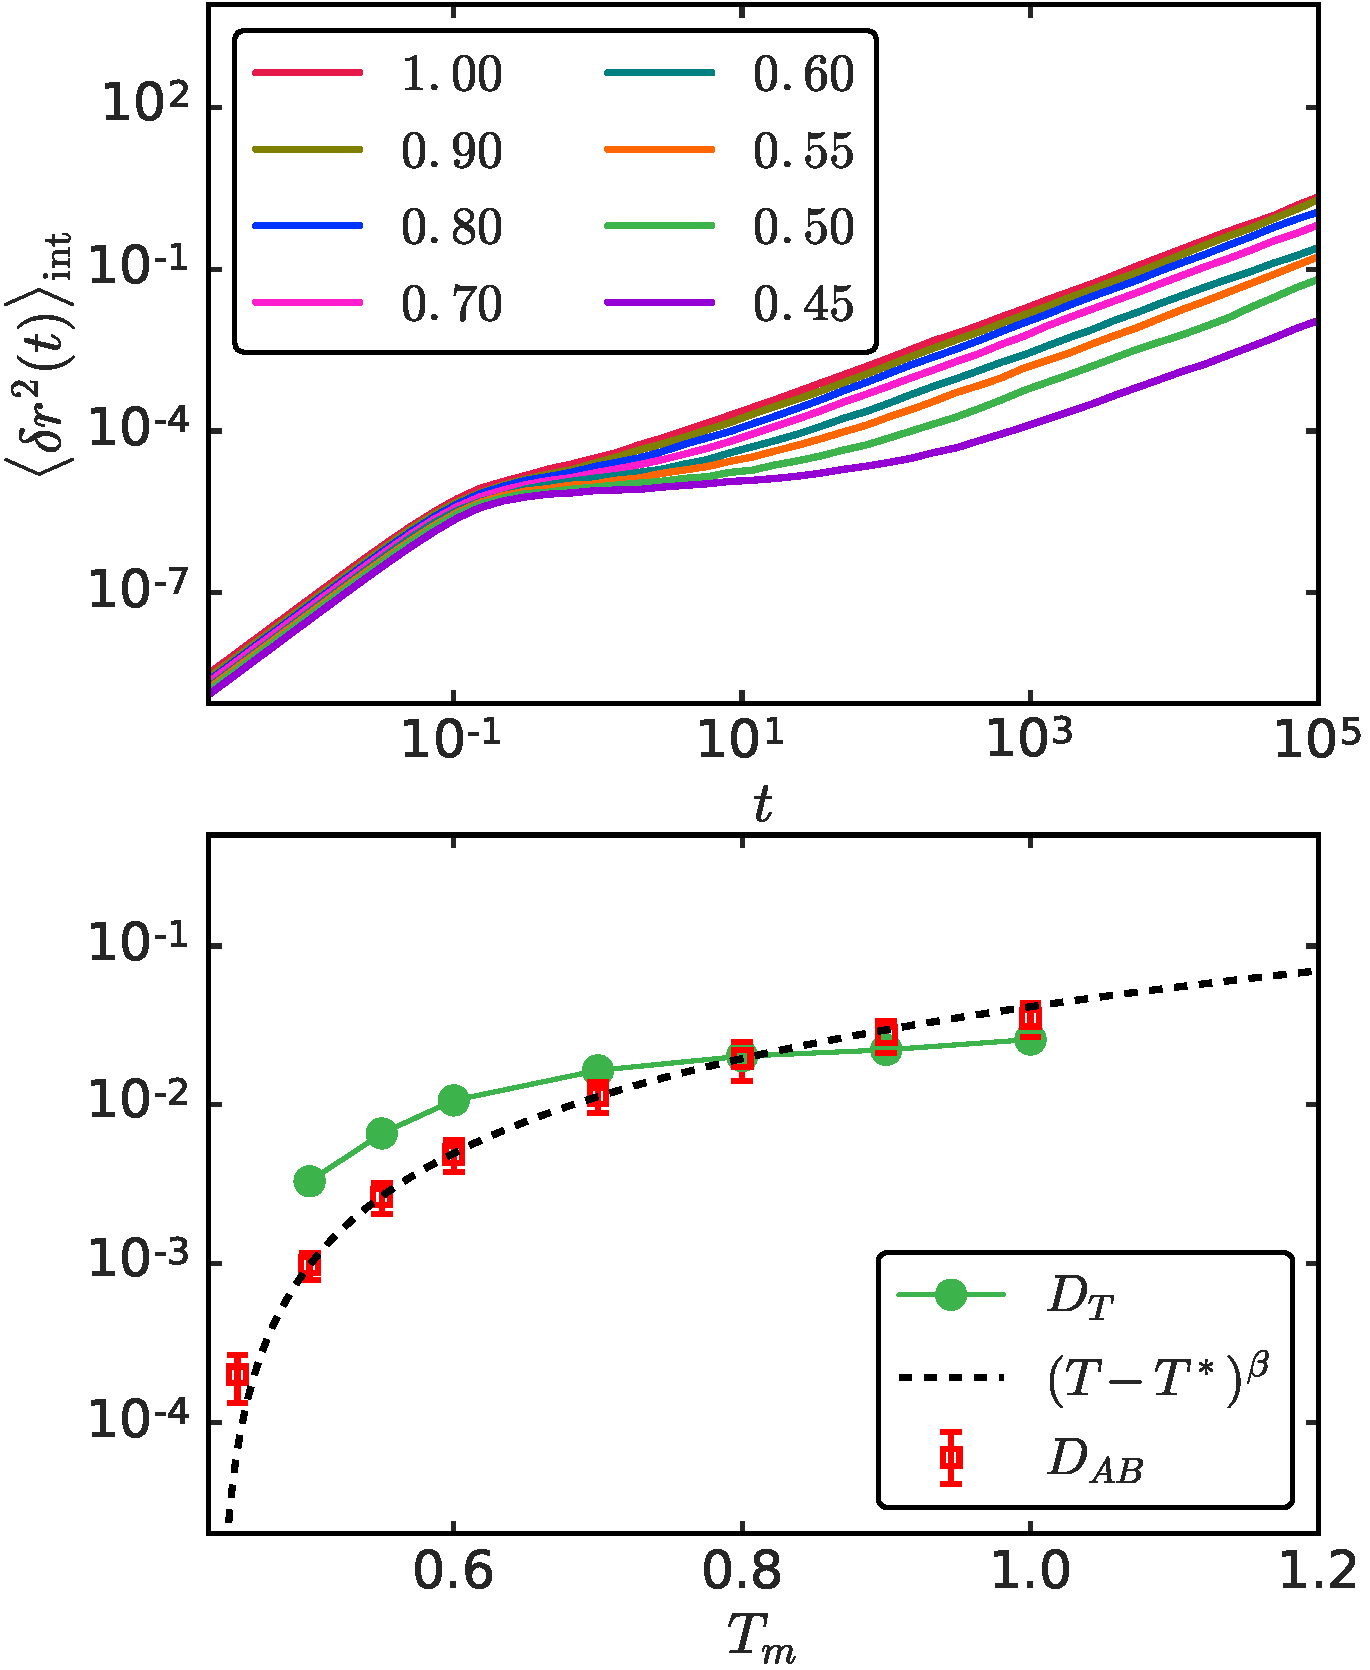
\includegraphics[width=12cm]{figs/fig3p3.pdf}
	\caption[{\em Center of mass MSD and interdiffusion coefficient measurement}]{(top) MSD of center-of-mass of A population, $\langle\delta{r^2(t)}\rangle_{\rm int}$, for different temperatures (as indicated) using equilibrium simulations. (bottom) Corresponding temperature variation of inter-diffusion coefficient $D_{AB}$ (shown with red squares) which behaves as $\sim(T-T^*)^{\beta}$ with $T^*=0.427$ and $\beta=1.8$ (shown with dashed line). Also shown is the estimate of thermal diffusivity $D_T$, from Soret coefficient, $S_T$, measured in non-equilibrium simulations, and $D_{AB}$: $D_T=S_T{D_{AB}}$. \label{fig3p3}}
\end{figure}

From the temperature dependence of the Soret coefficient, $S_T=D_T/D_{AB}$, we can infer that the thermal diffusivity becomes more dominant ($S_T > 1$) as we approach the glassy regime. Using equilibrium simulations, it is possible to measure the interdiffusion coefficient (also check section-\ref{selfInter} of Chapter-\ref{chap1} for detailed discussion on interdiffusion) $D_{AB}$ %from a generalized Einstein relation \cite{interdiff} in the following manner. 
by tracking the center of mass trajectory of the A species, ${\bf R}_A(t)=\frac{1}{N_{A}}\sum_{j=1}^{N_A}{\bf r}_j^{A}(t)$, and computing the corresponding mean squared displacement, $\langle\delta{r^2(t)}\rangle_{\rm int}=\langle[{\bf R}_A(t)-{\bf R}_A(0)]^2\rangle$, the data for which is shown in the top panel  of Fig.~\ref{fig3p3} for the range of temperatures explored. The interdiffusion coefficient can then be computed \cite{interdiff} via the "Einstein relation": $$D_{AB}=\lim_{t\rightarrow\infty}\Big{[}1+\frac{x_A}{x_B}\Big{]}^2\Phi{Nx_Ax_B}\frac{\langle\delta{r^2(t)}\rangle_{\rm int}}{6t},$$ where $\Phi$ is the thermodynamic factor, defined as $\Phi=x_Ax_B/S_{\rm cc}(q=0)$, $S_{\rm cc}(q)$ being  the concentration-concentration structure factor, computed using  the partial structural factors $S_{\rm AA}(q)$, $S_{\rm BB}(q)$, $S_{\rm AB}(q)$ via the expression  $S_{\rm cc}(q)=(1-x_A)^2S_{\rm AA}(q)+x_A^2S_{\rm BB}(q)-2x_A(1-x_A)S_{\rm AB}(q)$.  In the limit of  $q\rightarrow{\infty}$, $S_{\rm cc}(q)\rightarrow{x_A(1-x_A)}$. For the Kob-Andersen binary LJ mixture, $\Phi$ doesn't vary much within the temperature regime of our interest, and is $\approx 2.55$.

\begin{figure}[hbt!]
	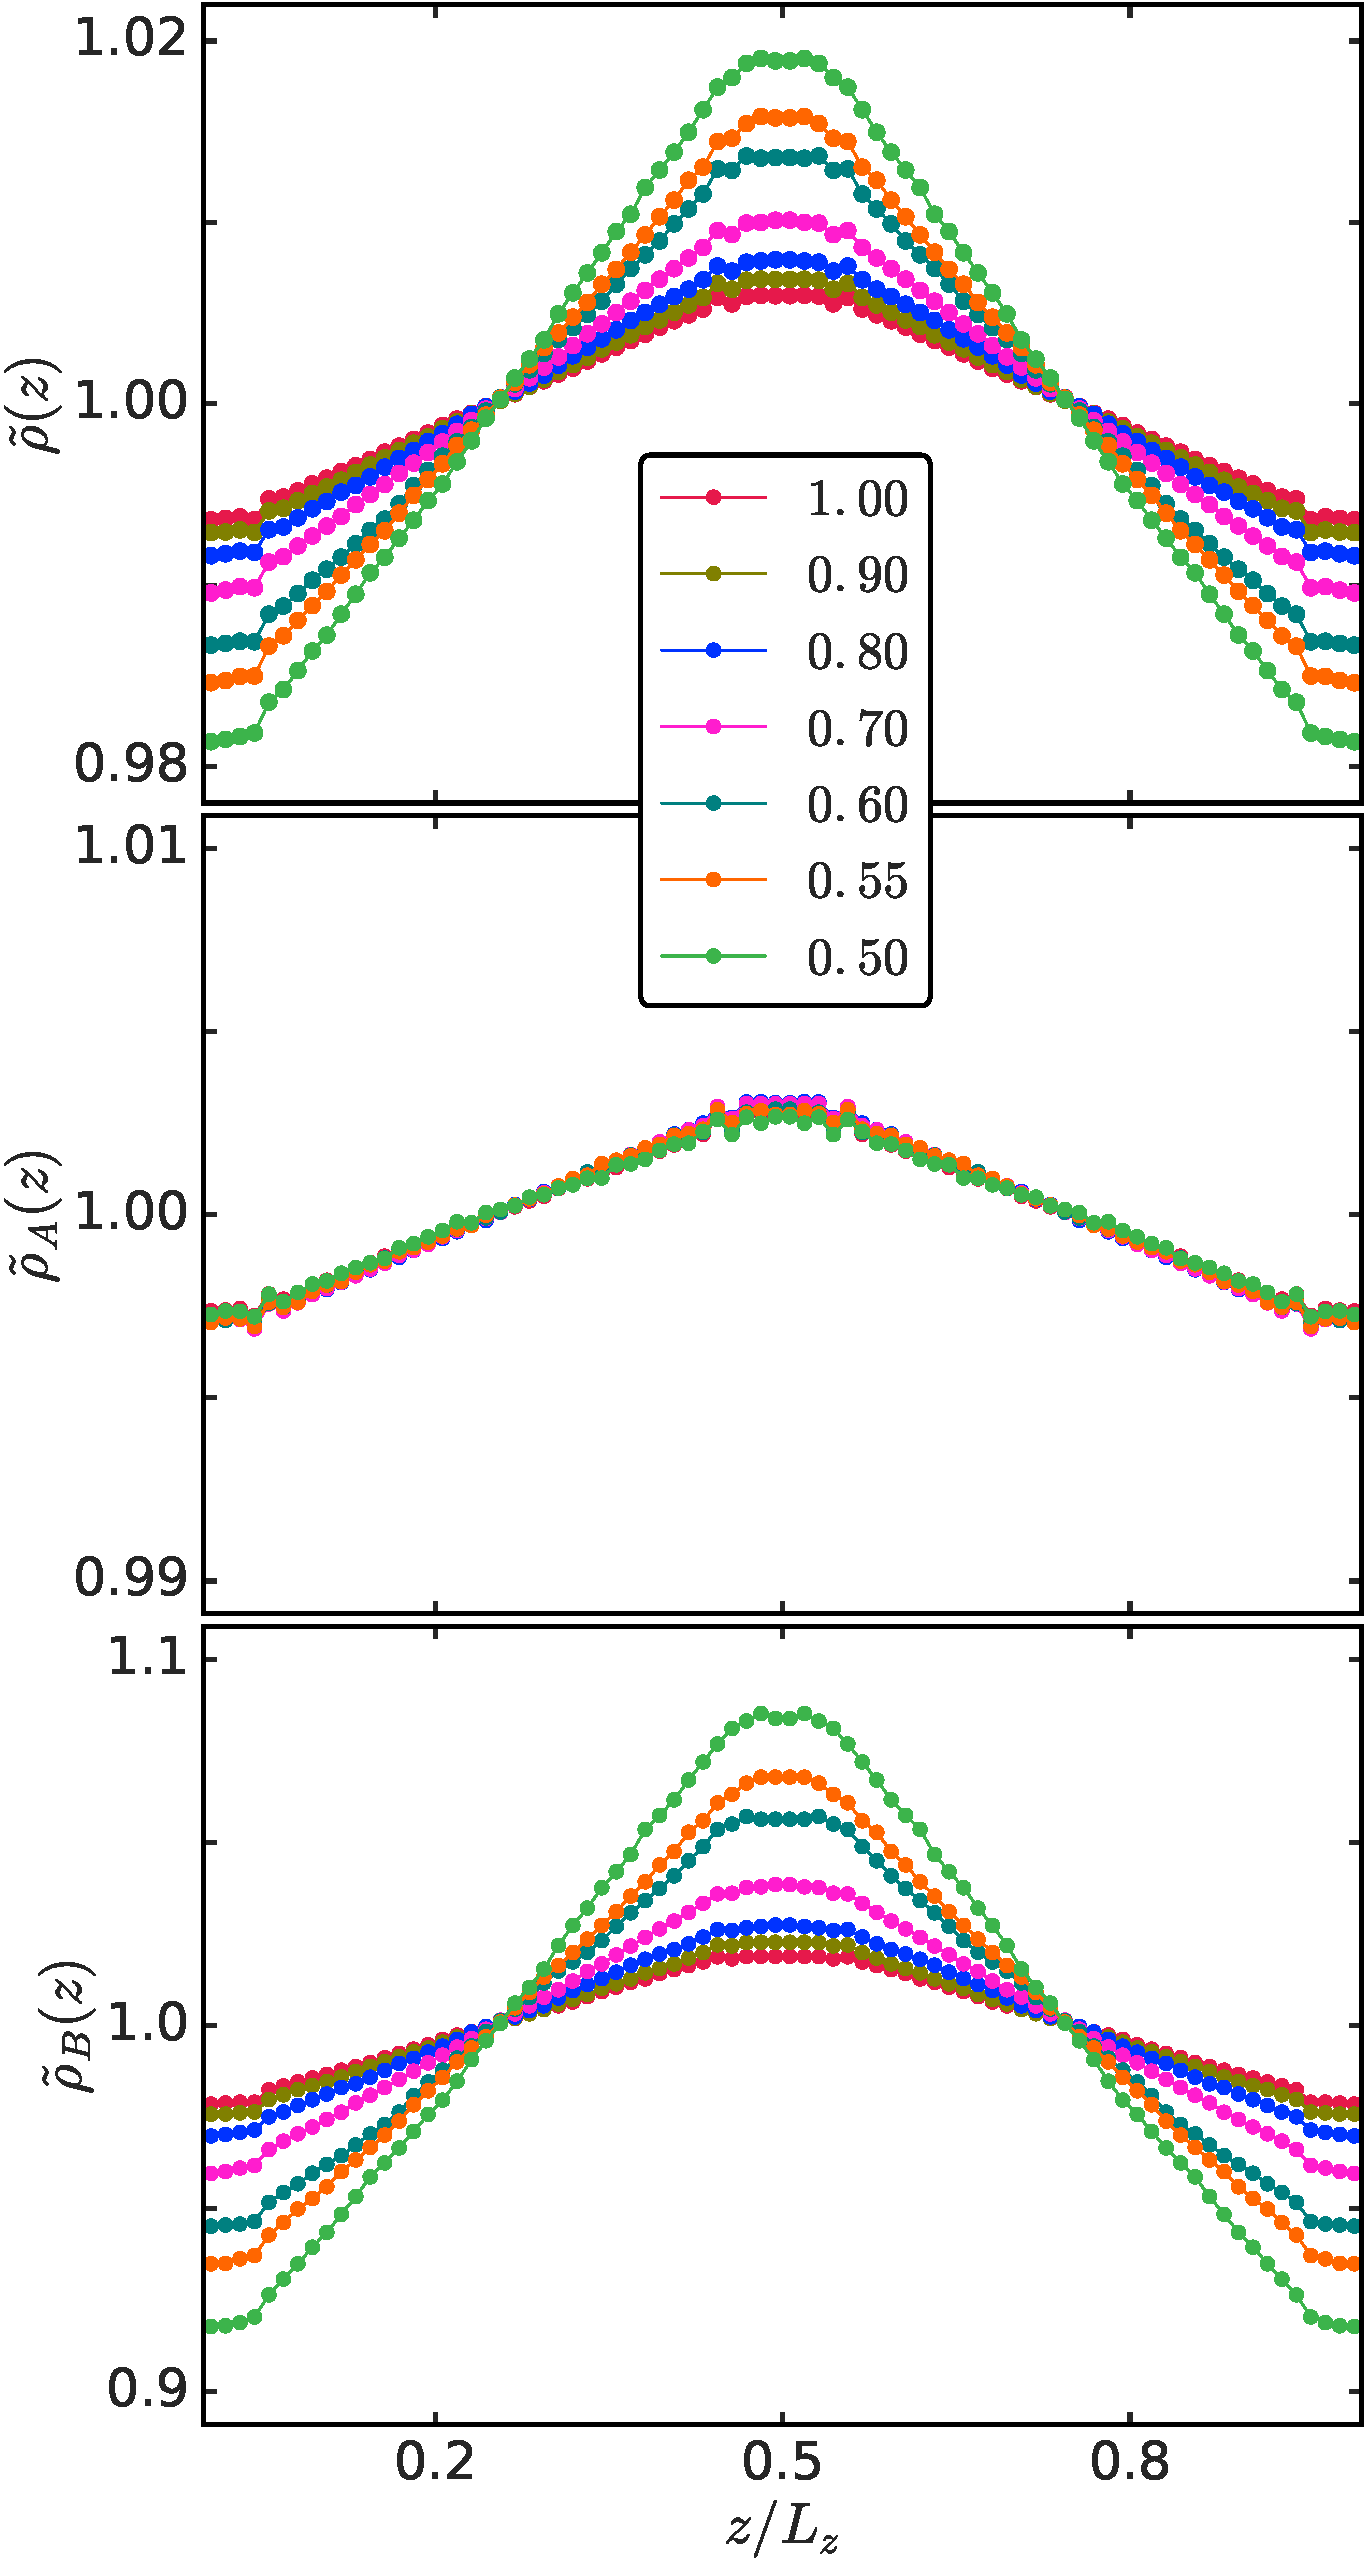
\includegraphics[width=11cm]{figs/fig3p4.pdf}
	\centering
	\caption[{\em Total density and partial densities profiles at different mean temperatures}]{For different values of $T_m$ (as marked), normalized density profiles (defined in text) for all particles (top) of A species (middle) and B species (bottom). \label{fig3p4}}
\end{figure}

The temperature dependence of the measured $D_{AB}$ is shown in Fig.~\ref{fig3p3} (bottom panel) and we demonstrate that the data can be fitted by $D_{AB} \sim (T-T^*)^{\beta}$, with $T^*=0.427$ and the effective exponent $\beta=1.8$. Thus, in the vicinity of $T_{\rm MCT}$ there is a drastic slowing down of this process and $D_{AB}$ would eventually vanish below the glass transition ($\approx{T_{VFT}}$). So we can infer from the behavior of the obtained Soret coefficient, that $D_T$, which characterizes the cross-correlation between thermal and mass flux, exhibits a slower decrease than the interdiffusive process, near $T_{\rm MCT}$ as we show in the bottom panel of Fig.~\ref{fig3p3}. {However, it also couples to the slow structural relaxation and thus one expects that $D_T$ vanishes below the glass transition temperature.} {In contrast, even when the supercooled liquid transforms to a glass, the thermal flux and thus the thermal conductivity is finite and decreases continuously \cite{bhuyan,mizuno}}.
%From various theoretical approaches in the framework of kinetic and mode-coupling theories \cite{goldhirsch83,piazza08,bringuier13}, we expect that, unlike the interdiffusion coefficient, $D_T$ is finite below the glass transition temperature, i.e.~for $T < T_{\rm MCT}$.

\begin{figure}[hbt!]
    \centering
	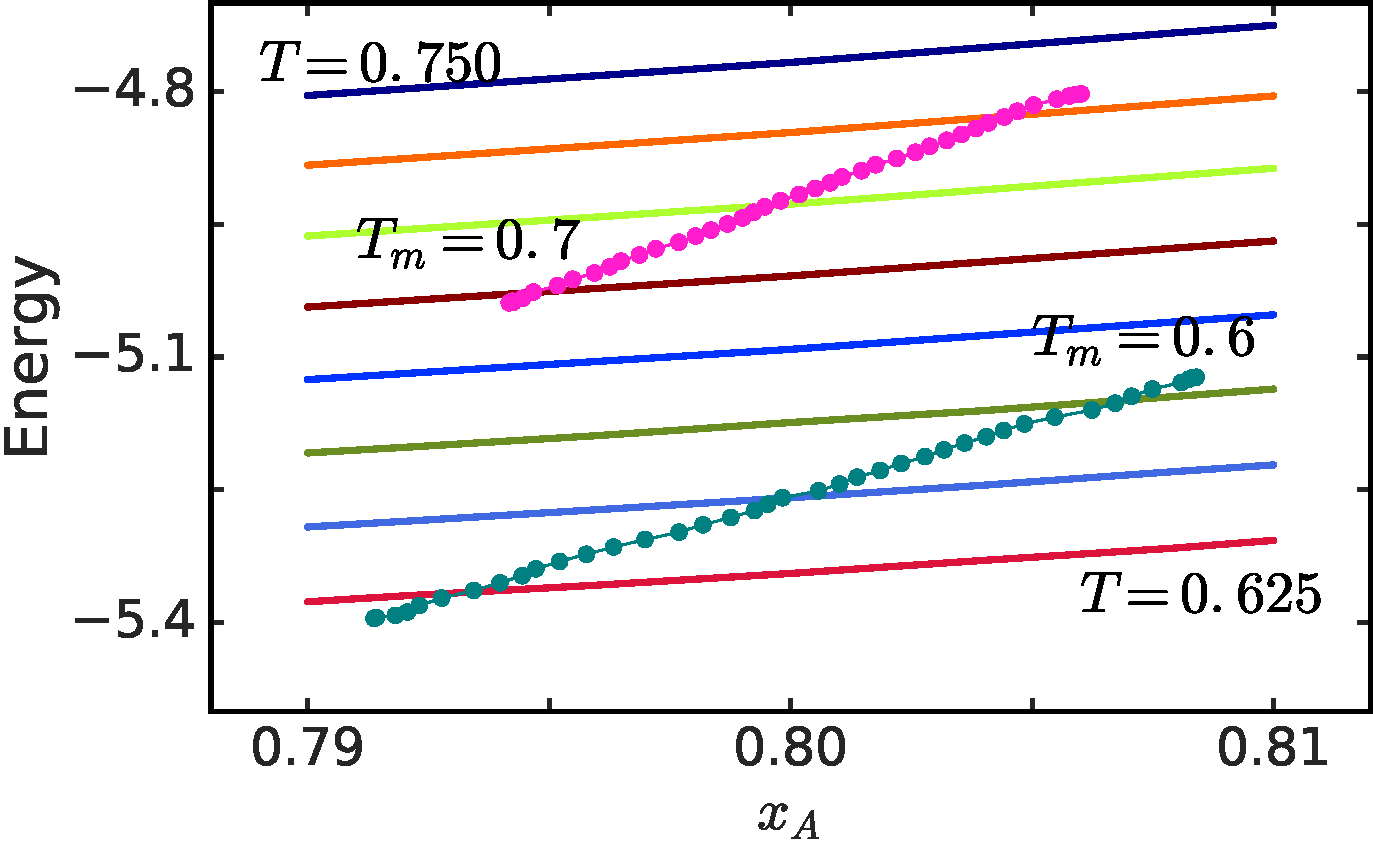
\includegraphics[width=12cm]{figs/fig3p5.pdf}
	\caption[{\em Confirming local equilibrium in steady state: local energy vs local concentration superposed on equilibrium isotherms}]{Local energy vs local concentration, shown for $T_m=0.6$ (cyan), $0.7$ (pink), superposed on equilibrium isotherms showing, for a range of temperatures, variation of energy with concentration. \label{fig3p5}}
\end{figure}

The spatial variation in concentration is associated with a variation of the density of each species, as shown in Fig.~\ref{fig3p4}(middle) and Fig.~\ref{fig3p4}(bottom) in terms of normalized density profiles of each species, $\tilde{\rho}_A(z)\equiv\rho_A(z)/\bar{\rho}_A$ and $\tilde{\rho}_B(z)\equiv\rho_B(z)/\bar{\rho}_B$, respectively, with $\bar{\rho}_A$ and $\bar{\rho}_B$ the total densities of A and B particles. For both species, the local density is higher at regions where the temperature is lower, {and similar  is the case with the overall density (see Fig.~\ref{fig3p4}(top) which is in agreement with} previous observations for a one-component fluid \cite{baranyai}. {However, there is also a difference in the response of the two species, such that the enhanced migration of the minority B species to the cold region results in the minimisation of the system's total energy and the enhancement of chemical order \cite{cargill}. This is evidenced in Fig.~\ref{fig3p5}: the emergent concentration profile is such that local equilibrium is satisfied, i.e., for the obtained combination of local $x_A$ and $T(z)$, the local energy measured from non-equilibrium simulations matches with the equilibrium value. The concentration gradient increases when $T_m$ approaches $T_{\rm MCT}$, while maintaining local equilibrium, as demonstrated via the comparative behaviour for $T_m=0.6$ and $T_m=0.7$ in Fig.~\ref{fig3p5}, with the decrease in local temperature leading to lower local energies and a wider range of $x_A$, via an increased affinity between the A and B species. This is manifested} in the increasing density variation, locally, of the minority B species, with decreasing $T_m$ [Fig.~\ref{fig3p4}(bottom)], while the spatial variation of $A$ species almost remains same [Fig.~\ref{fig3p4}(middle)].

We note here that the timescales for the migration of particles over large length scales leading to the emergence of the steady-state density profiles, and thereby the concentration profiles, strongly increase, as local temperatures approach the glassy regime. Thus, for all temperatures in the vicinity of $T_{\rm MCT}$, steady state conditions for the concentration profiles become difficult to attain, which we discuss below. This slowness contrasts the fast onset of the steady thermal current, which results in anomalies, as further elucidated later.

\subsection{Supercooled liquid: nonlinear response} 

%
\begin{figure}[hbt!]
    \centering
	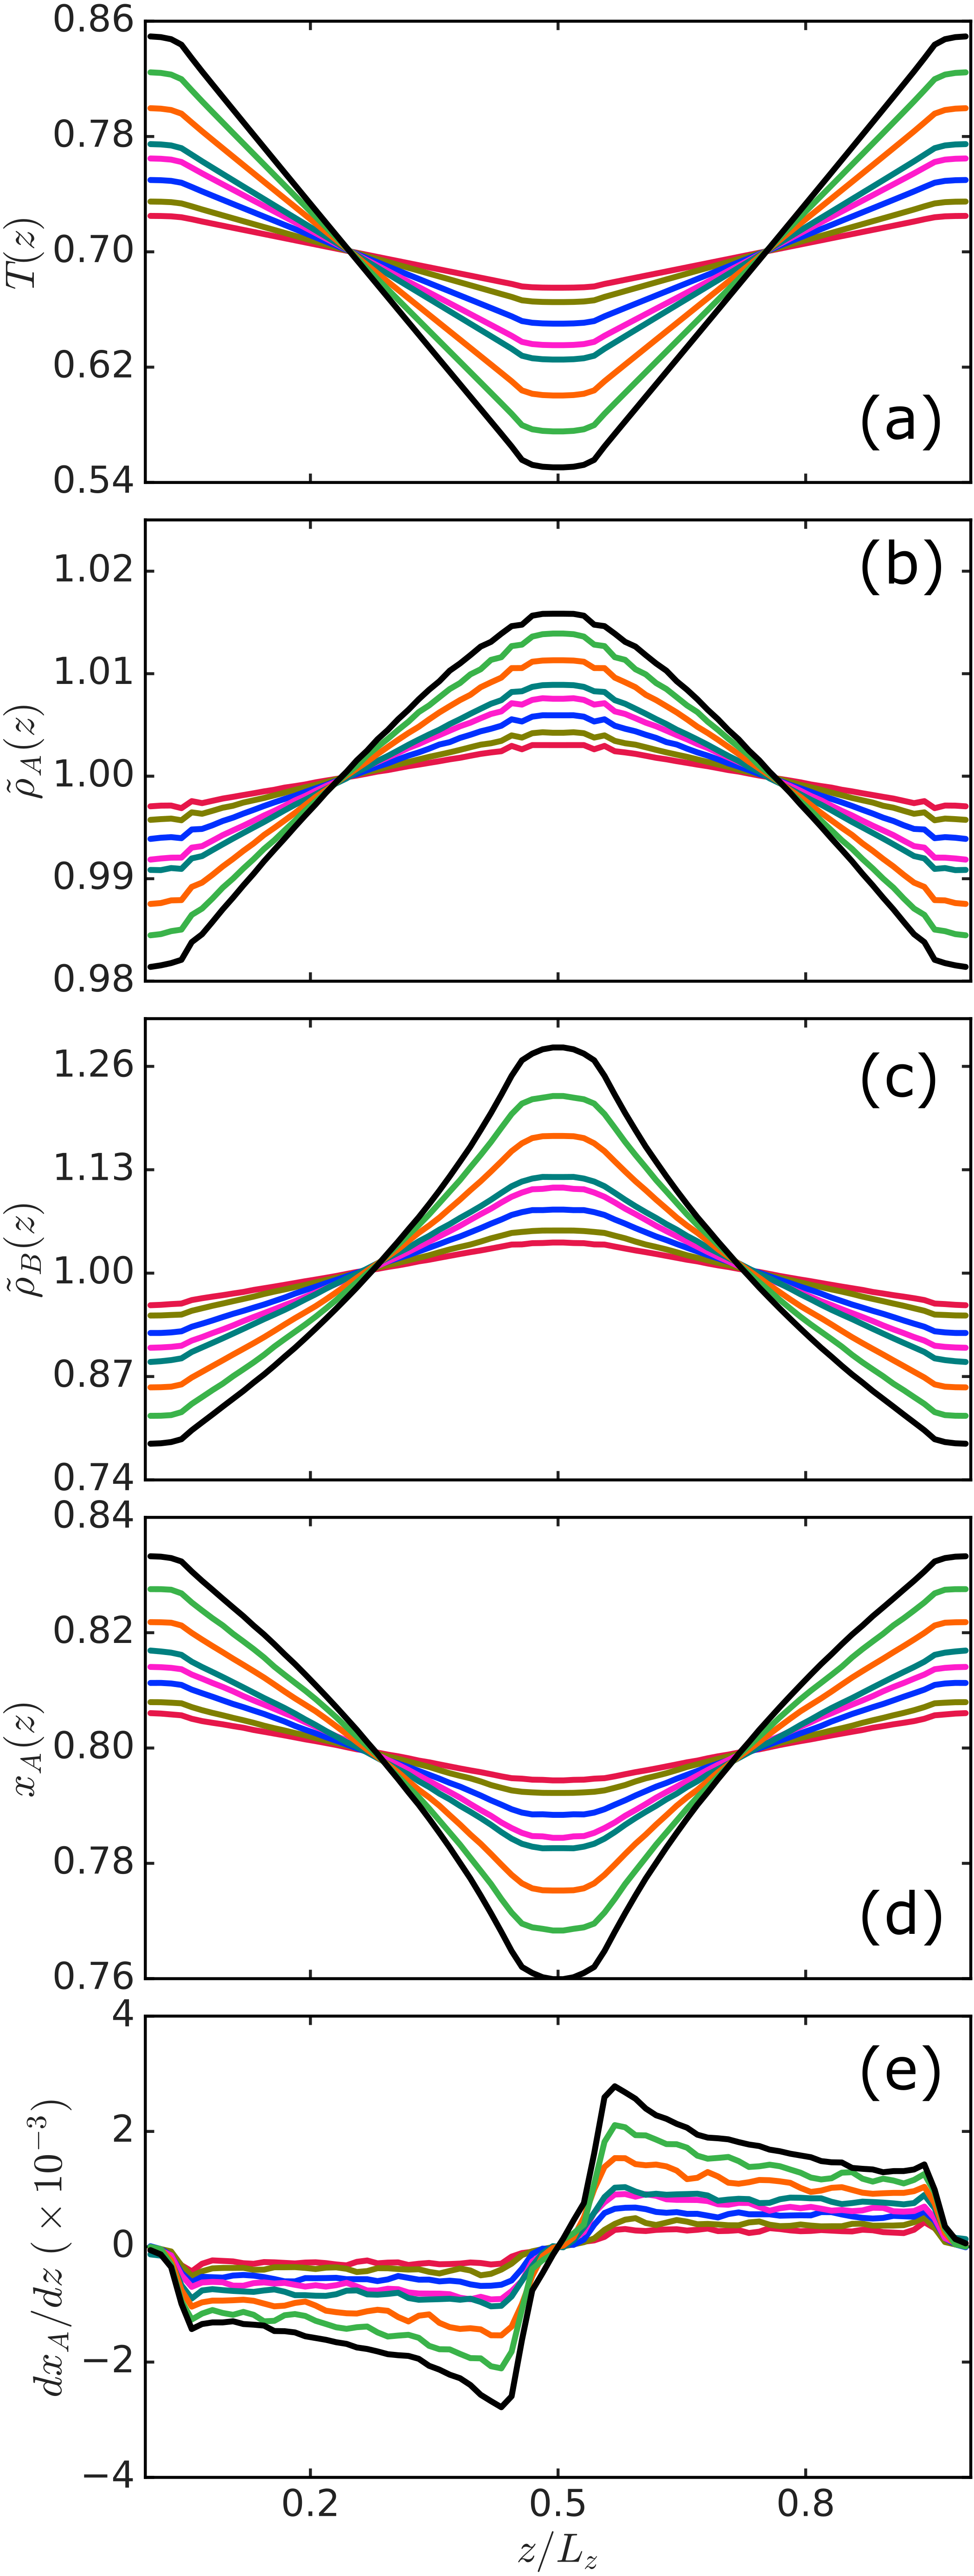
\includegraphics[width=7cm]{figs/fig3p6.png}
	\caption[{\em Varying gradient strength at $T_m=0.7$, to observe linear and nonlinear response}]{$T_m=0.7$: (a) Temperature profiles, $T(z)$, for increasing applied thermal gradient, shown for $(dT/dz)10^3=1.33, 1.86, 2.66, 3.45, 3.99, 5.31, 6.64, 7.97$. Corresponding normalised density profiles of A species (b), B species (c). (d) Concentration profiles of A particles; (c) gradient of the concentration profiles shown in (d). \label{fig3p6}}
\end{figure}

%%
\begin{figure}[hbt!]
    \centering
	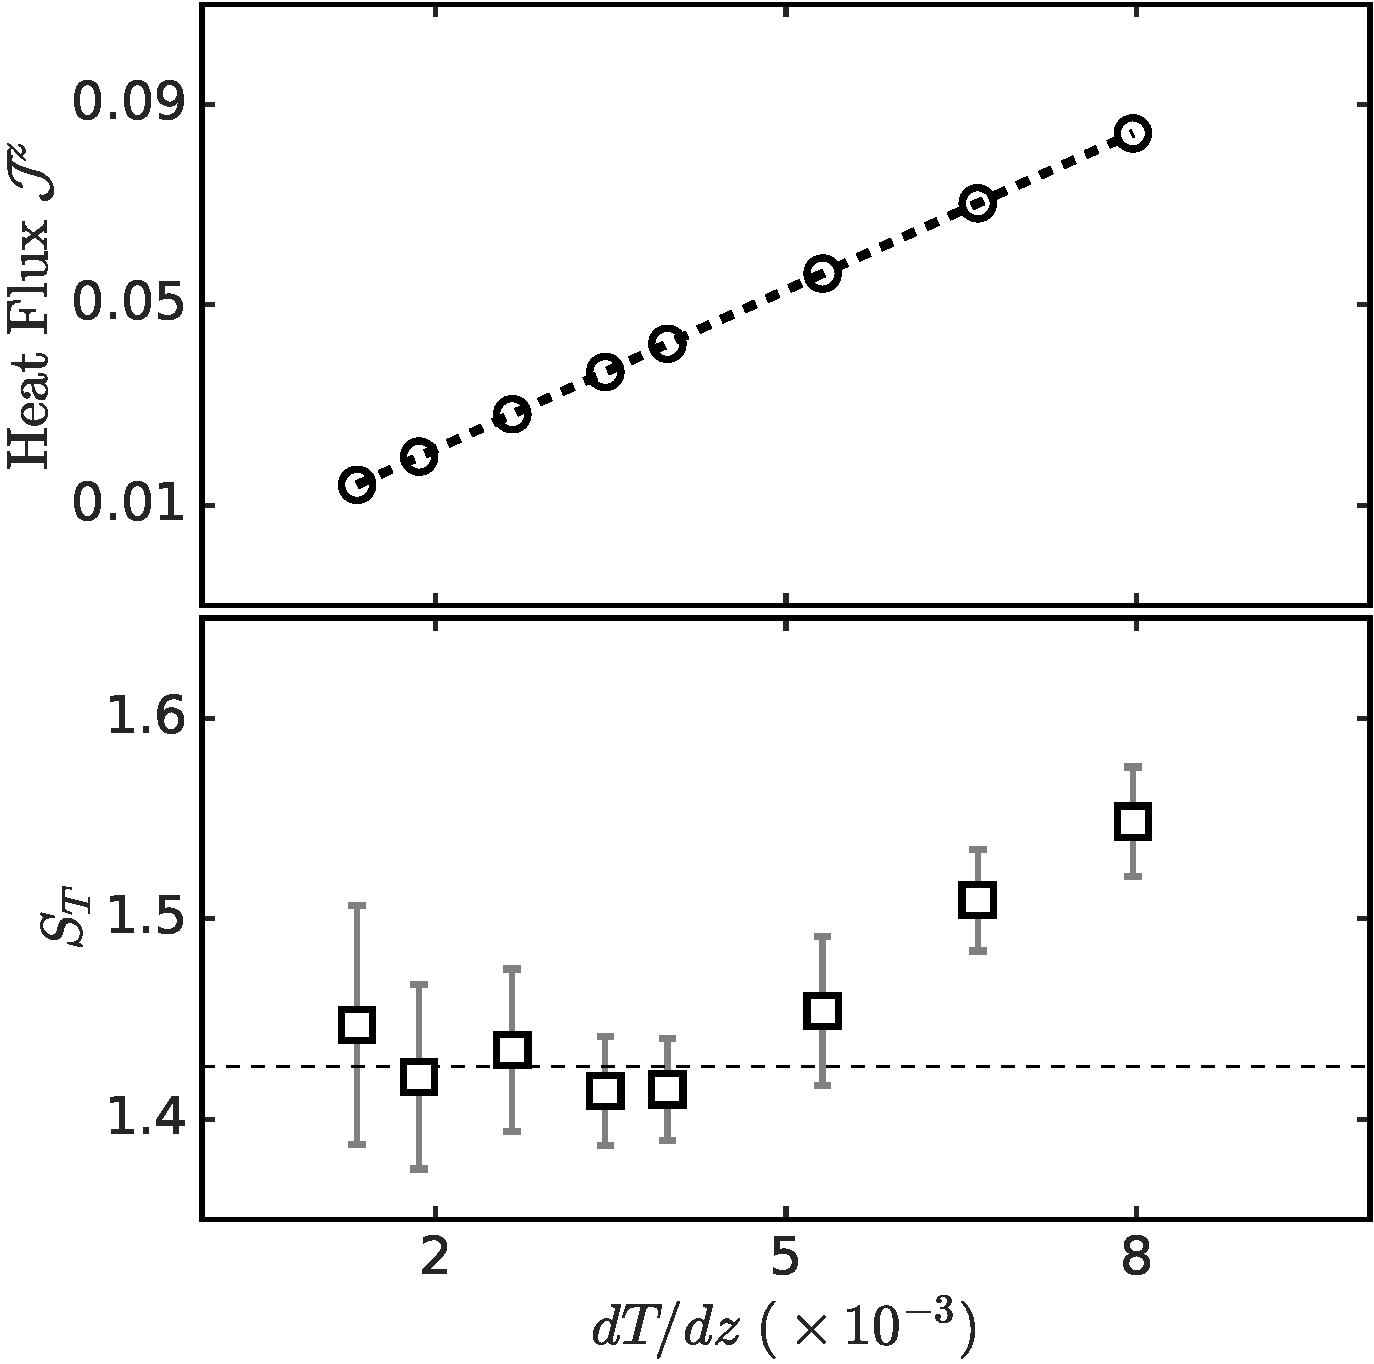
\includegraphics[width=12cm]{figs/fig3p7.pdf}
	\caption[{\em Heat flux and Soret coefficient as function of temperature gradient at $T_m=0.7$}]{$T_m=0.7$. (Top) Variation of heat flux $J^z$ with changing imposed temperature gradient ($dT/dz$): linearity is maintained over the entire range of applied gradients.$S_T$ computed from the temperature and concentration profiles shown in  Fig.~\ref{fig3p3} (a), (d). (Bottom) The dashed line corresponds to the average value of $S_T$ in the linear response regime.\label{fig3p7}}
\end{figure}

\begin{figure}[hbt!]
    \centering
	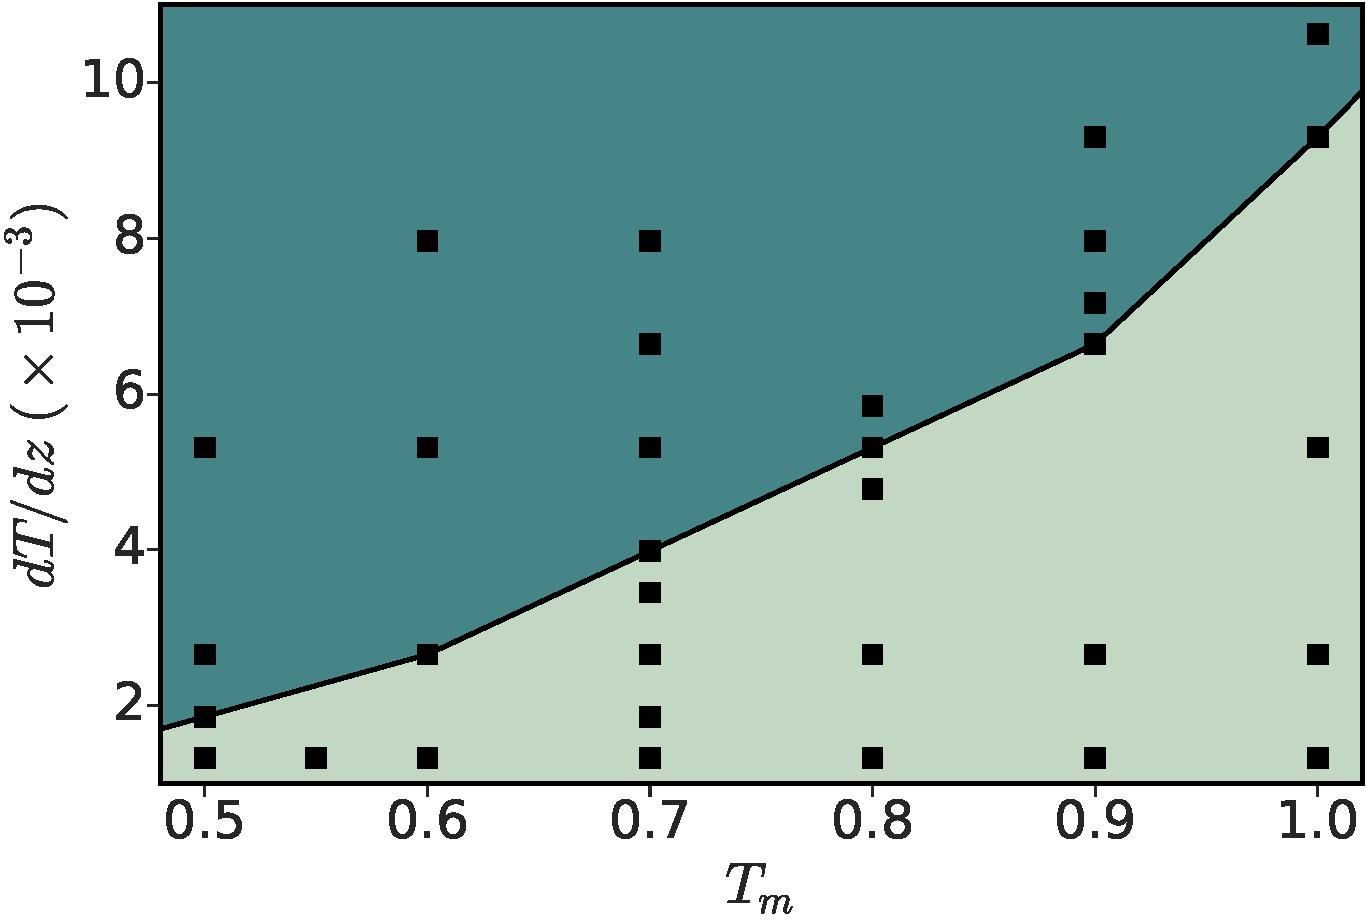
\includegraphics[width=12cm]{figs/fig3p8.pdf}
	\caption[{\em State diagram in the $\{T_m, dT/dz\}$ plane, indicating linear and nonlinear response}]{State diagram in the $\{T_m, dT/dz\}$ plane, indicating where the transition from linear response (light-green area) to nonlinear response (dark-green area) sets in.\label{fig3p8}}
\end{figure}
%
\begin{figure}[hbt!]
    \centering
	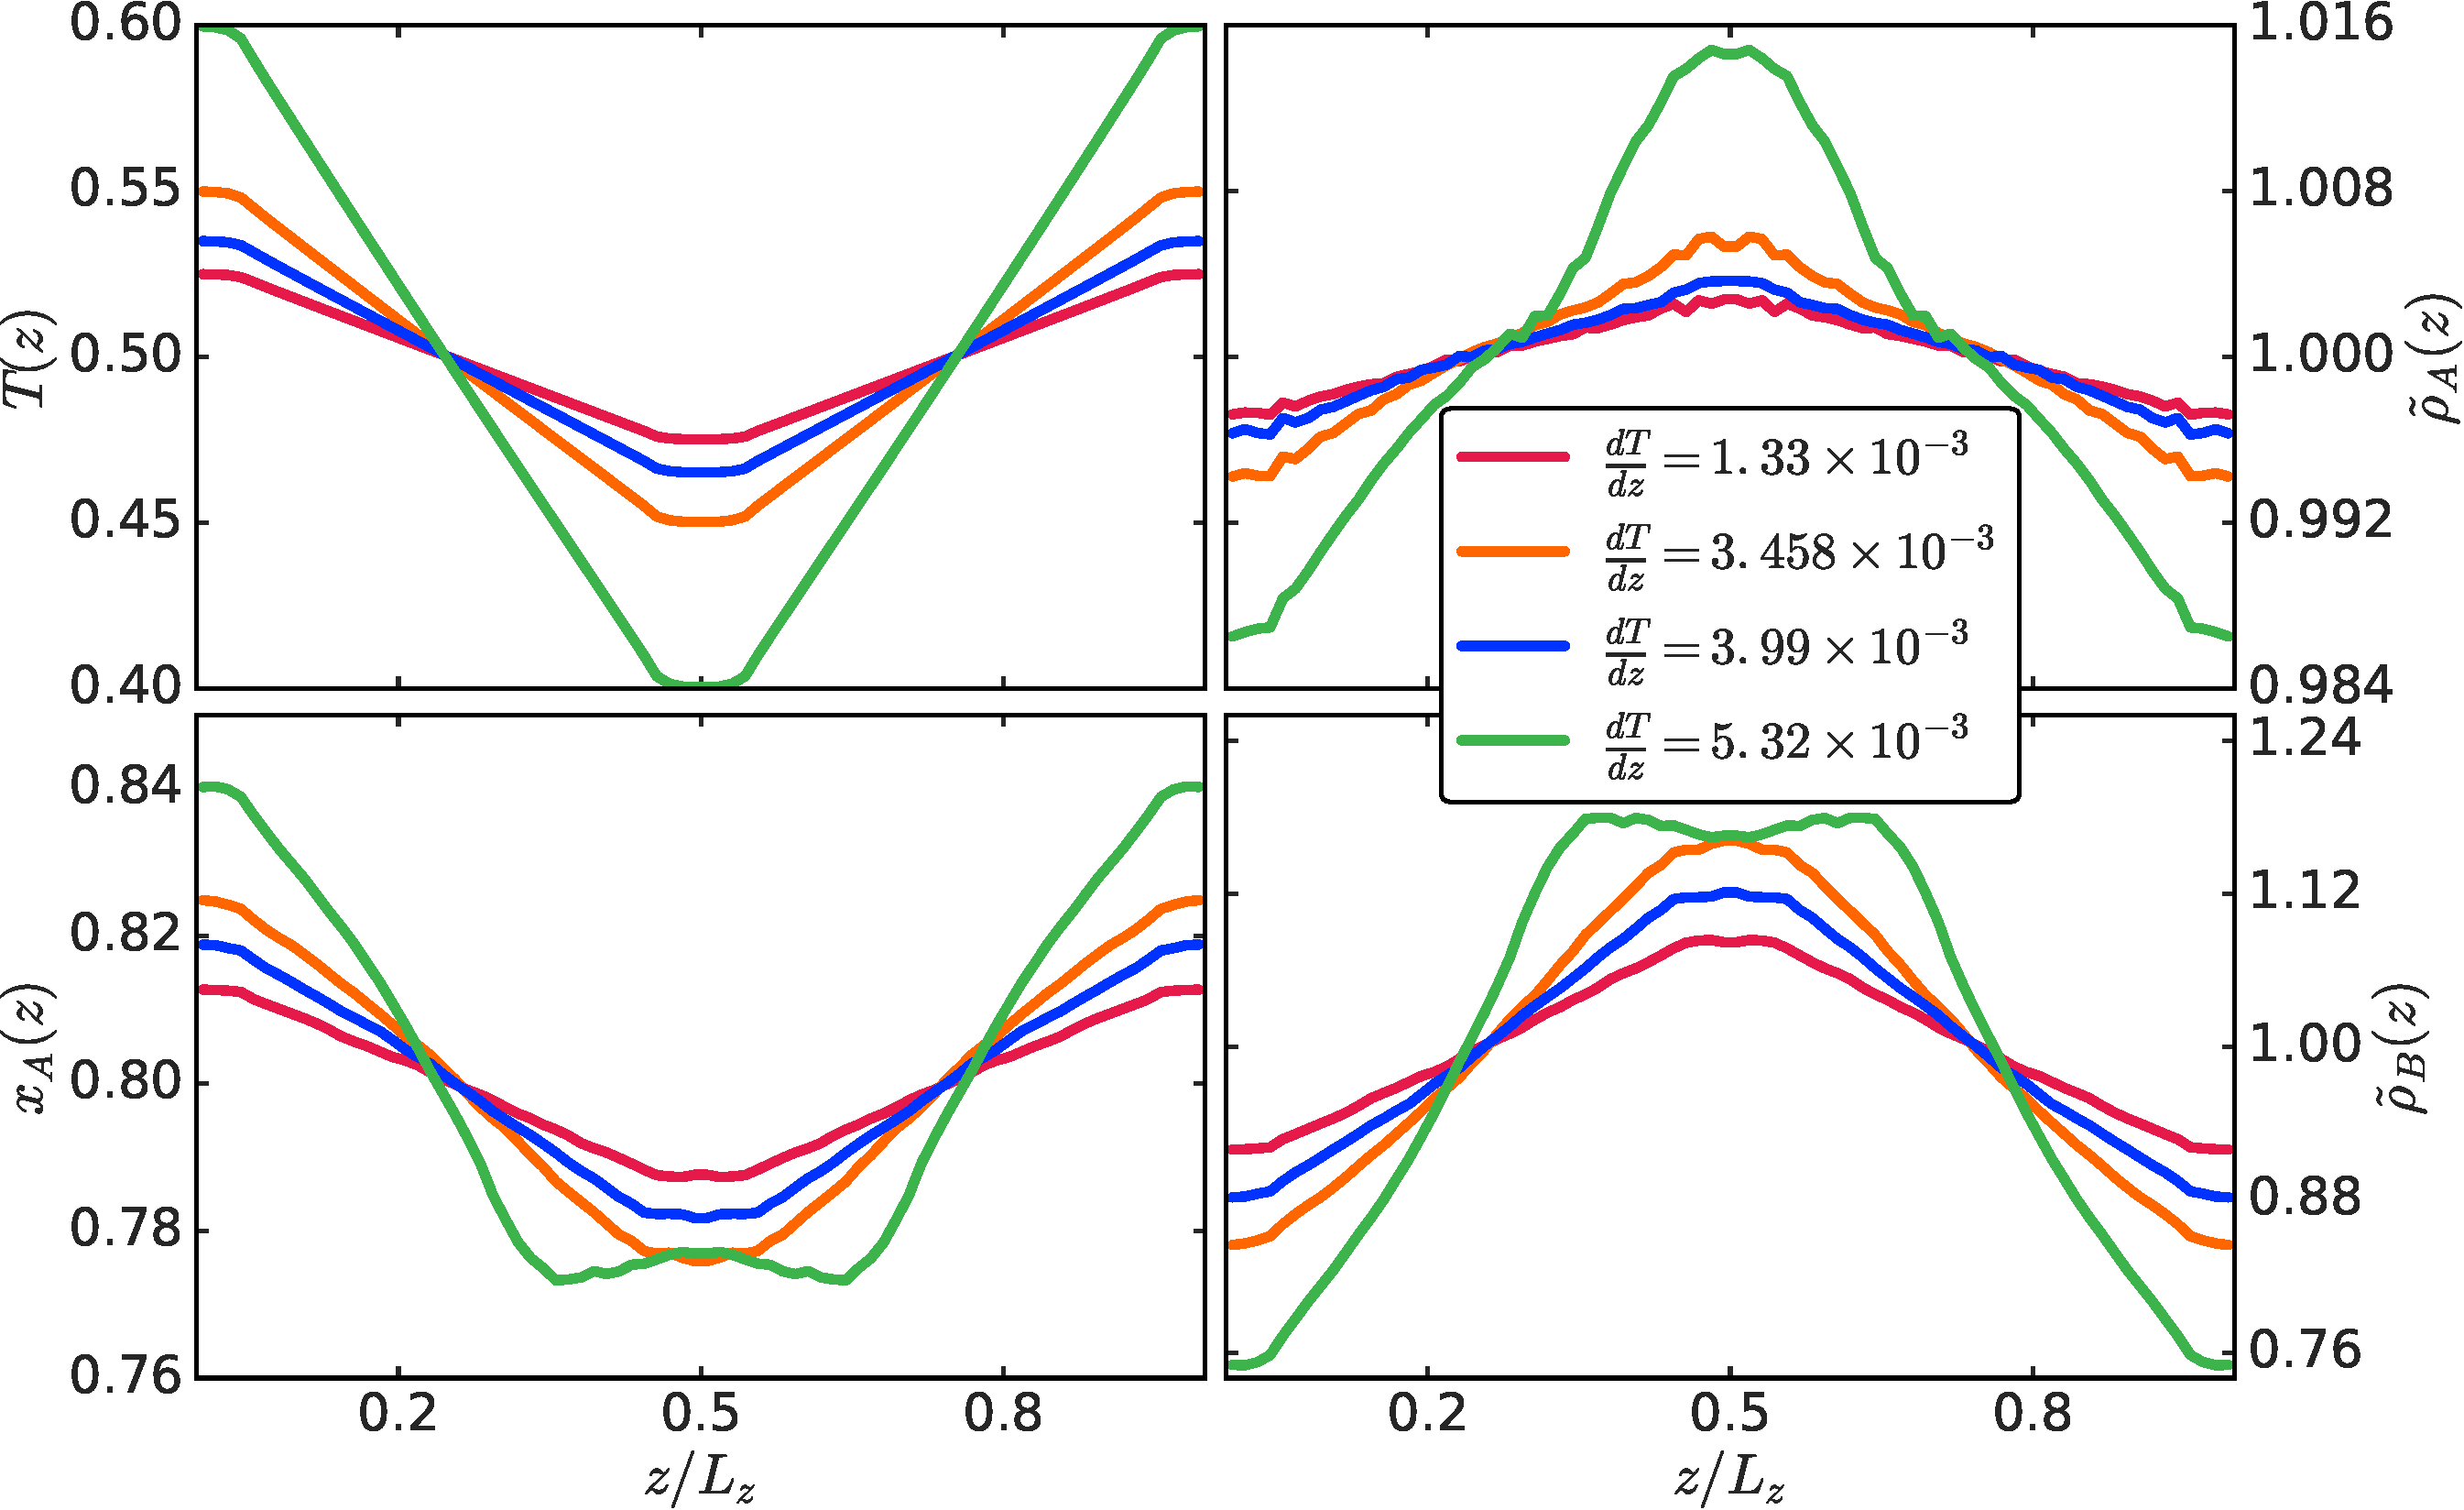
\includegraphics[width=15cm]{figs/fig3p9.pdf}
	\caption[{\em Thermal response at $T_m=0.5$}]{$T_m=0.5$. (Left) Profiles of temperature (top) and concentration of A particles (botttom), for increasing applied gradient ($dT/dz$). (Right) Corresponding profiles of local density of A (top) and B (bottom) particles, normalized with the respective global density.\label{fig3p9}}
\end{figure}

We now explore the question of how the concentration profiles change when the applied thermal gradient, $dT/dz$, is varied. In Fig.~\ref{fig3p6}(a)-(e), we illustrate the case for $T_m=0.7$.  For all considered values of $dT/dz$, a linear temperature profile [Fig.~\ref{fig3p6}(a)] and a linear dependence of the corresponding heat current on $dT/dz$ (see Fig.~\ref{fig3p7}(top)), implying that the thermal response is within the linear regime.  However, the corresponding concentration profiles for A particles, $x_A(z)$, are linear at small $dT/dz$ and become more and more nonlinear as $dT/dz$ increases [Fig.~\ref{fig3p6}(d)]. This is evident from the spatial profiles of the concentration gradient, $d{x_A}/dz$, as shown in Fig.~\ref{fig3p6}(e) -- constant for small gradients and otherwise with increasing gradient.  We emphasise that these profiles are observed in the steady-state and do not reflect any transient behaviour. The departure from the linear response is also seen in the dependence of the Soret coefficient (the local slope is calculated over 7 bins) with increasing thermal gradient in Fig.~\ref{fig3p7}(bottom). While it is constant at sufficiently small values of $dT/dz$, it starts to increase at a gradient of about $dT/dz\approx 5\times 10^{-3}$. Microscopically, the nonlinear response is associated with a stronger enrichment of the B species at the colder region (cf.~the difference in response of density profiles of A and B species with increasing gradient; see Fig.~\ref{fig3p6}(b),(c)).

From the behavior of $d{x_A}/dz$, we chart out the transition from linear to nonlinear response for the various $T_m$ in the supercooled liquid in Fig.~\ref{fig3p8}.  Here, the important finding is that the linear response regime breaks down at smaller and smaller thermal gradients with decreasing temperature.  Such temperature dependence of nonlinearities is reminiscent of the mechanical response of supercooled liquids \cite{ludo,zausch}, where similar nonlinear effects are observed at increasingly smaller forcing with decreasing ambient temperature.

{We note that in the vicinity of $T_{\rm MCT}$, with increasing gradient, local temperatures in the cold region start to fall below $T_{\rm MCT}$. We show one such example in Fig.~\ref{fig3p9}, where for $T_m=0.5$ and the largest applied gradient, the local temperature goes below $T_{\rm MCT}=0.435$ and consequently steady-state behaviour is not obtained within the observed time-window.}

%
\subsection{Response at mean temperature below VFT-temperature}

Having so far explored the response of supercooled liquids, we now consider the case $T_m=0.2$ which is below $T_{\rm VFT}\approx{0.3}$, i.e.~in the glassy regime where relaxation processes are very slow or nearly arrested.  If we impose $\Delta{T}=0.05$, very soon, a linear temperature profile sets in, and there is a finite heat current between the hot and cold regions; see Fig.~\ref{fig3p10}(left). Note that for the applied $\Delta{T}$, all local regions are in the glassy state. Here, unlike the liquid regime, the concentration profile shows no spatial dependence and, for all waiting times after application of the thermal gradient, it is nearly indistinguishable from the one measured for the quiescent aging glass [Fig.~\ref{fig3p10}(right-down)].  Thus, for the glass, under applied thermal gradient, the local concentrations remains intact, under applied thermal gradient, i.e.~the Soret effect is not observed. The density profiles of each species (see Figs.~\ref{fig3p10} (right-top, right-middle)) evidence that the majority component, i.e.~the A particles, do respond to the thermal gradient, albeit with very small changes in local density due to a local expansion of the volume.  In contrast, over the time scale of the observation, the B particles are nearly unresponsive.  Or, in other words, the reorganization of the minority species, that is necessary for any concentration variation to happen, as demonstrated earlier, is not induced via the applied thermal gradient, where locally all regions are in the glassy regime.

%
\begin{figure}[hbt!]
    \centering
	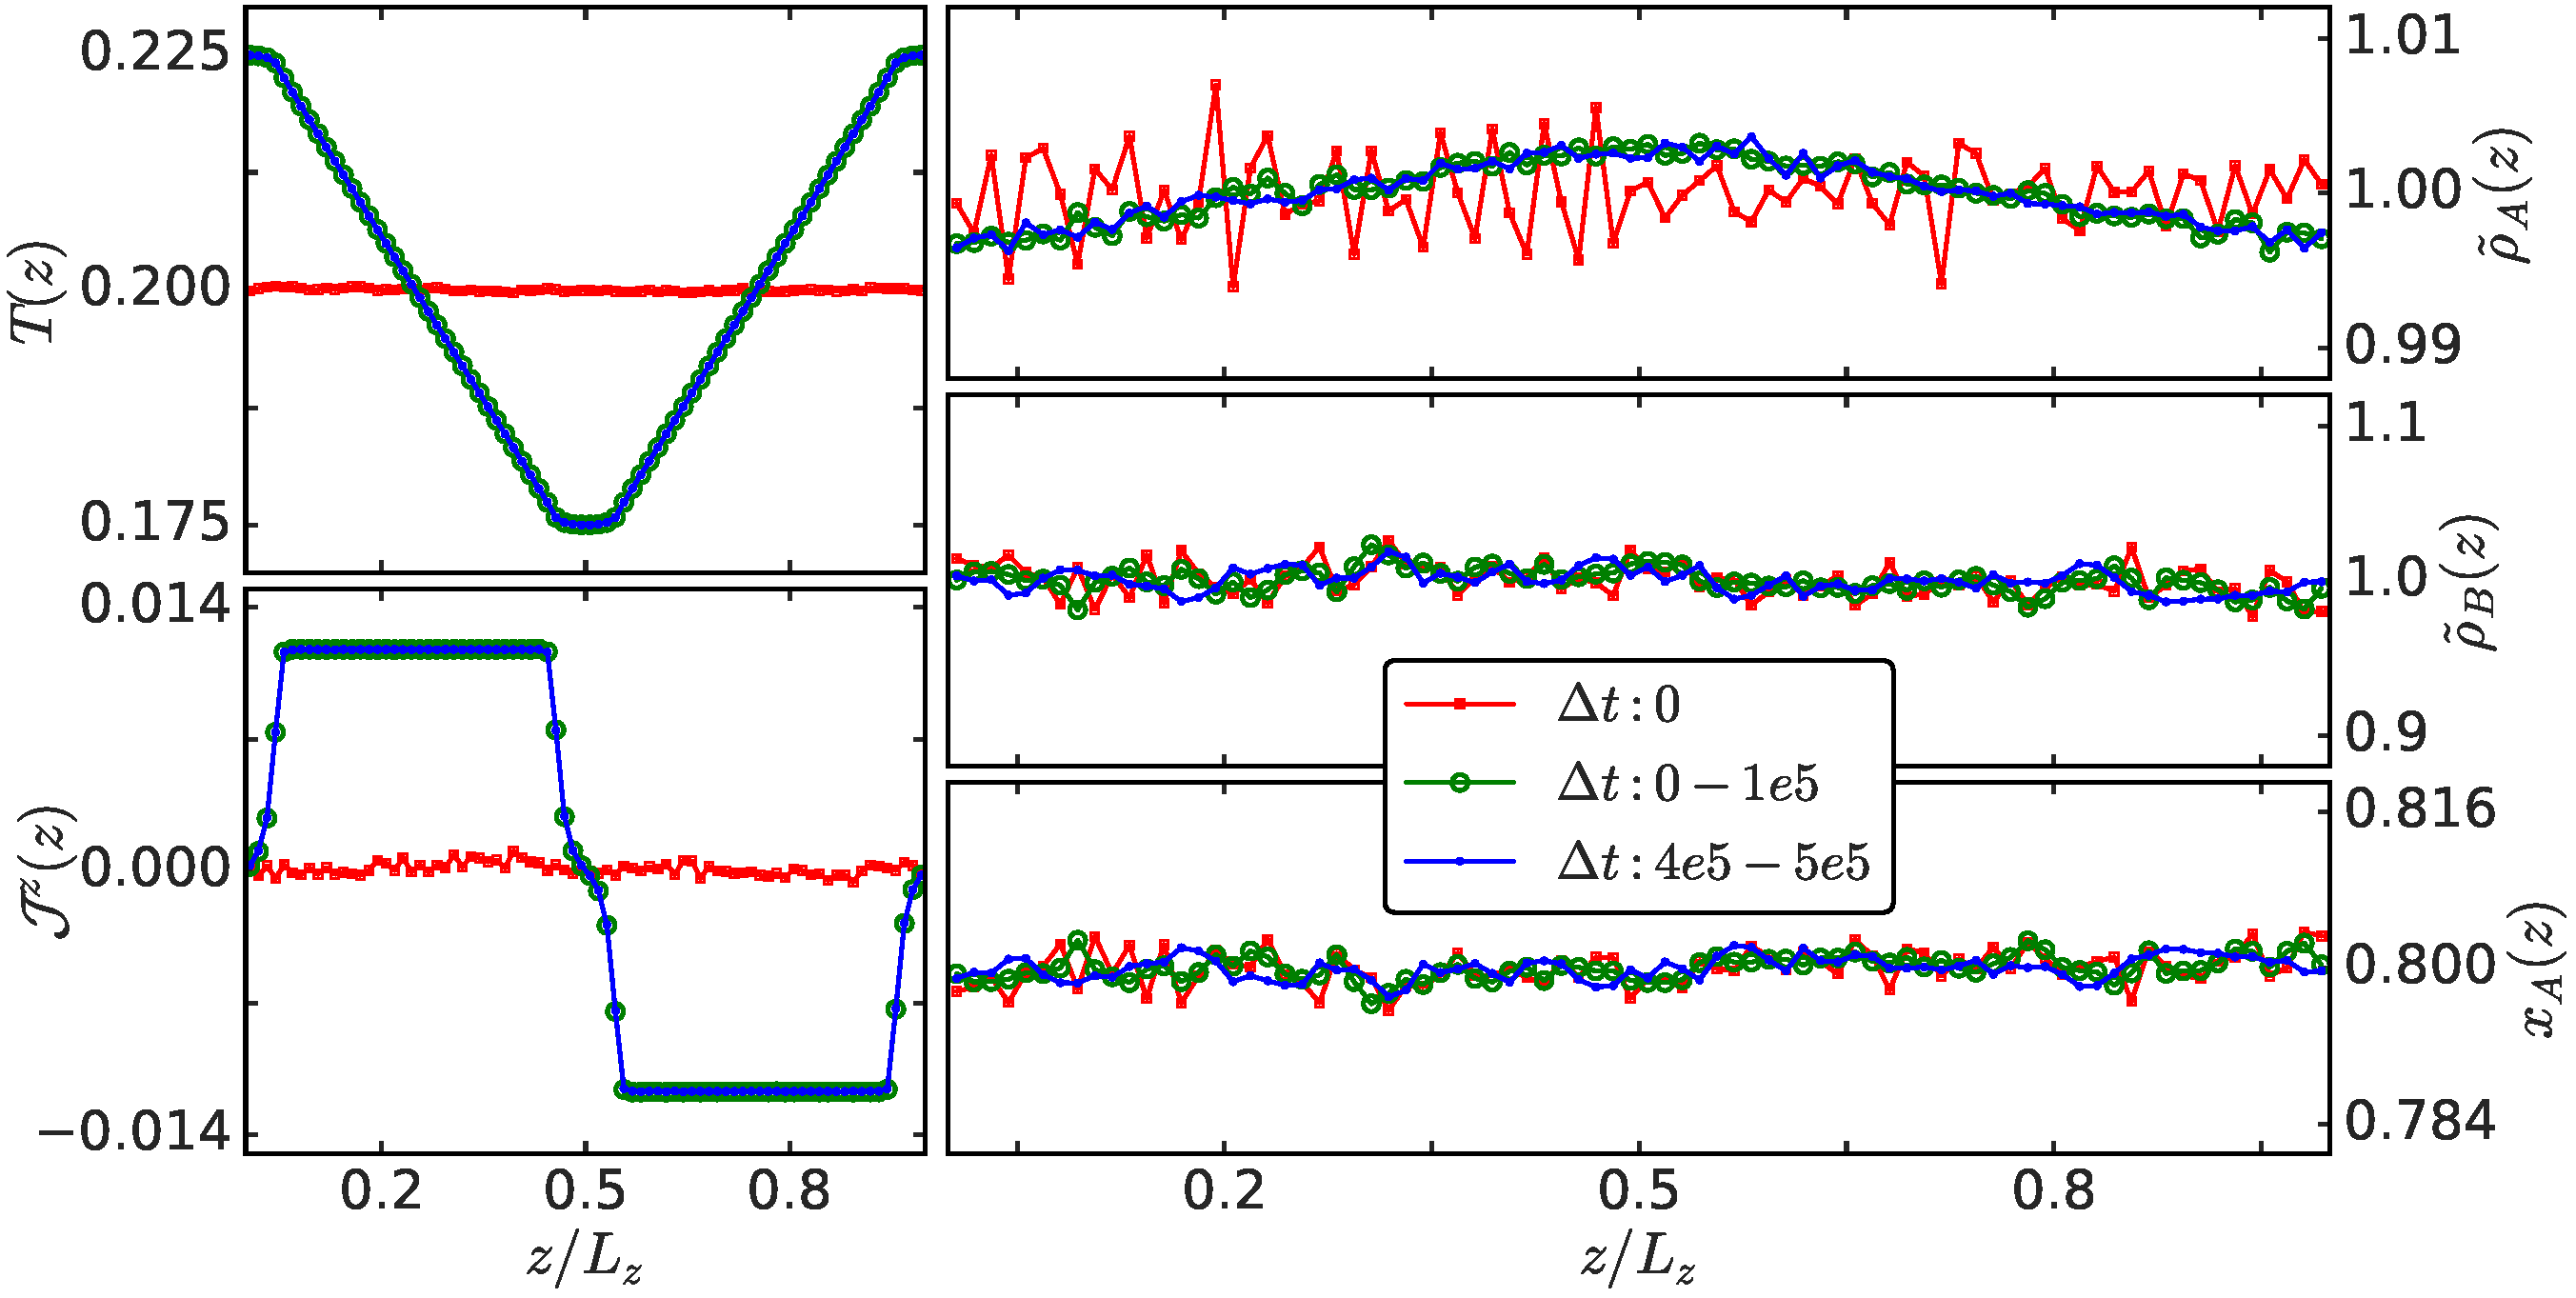
\includegraphics[width=15cm]{figs/fig3p10.pdf}
	\caption[{\em Thermal response at $T_m=0.2$}]{$T_m=0.2$.$\Delta{T}=0.1$;. (Left) Spatial profile of (top) applied thermal gradient and (bottom) corresponding heat current that develops. (Right) Evolution of spatial profile of normalized density of A species (top), B species (middle) and concentration of A species (bottom), {shown for  different time windows $\Delta{t}/10^5=0-$1(blue), $4-5$(green)}. Corresponding data for unperturbed system at $T=0.2$ are shown as dashed lines. \label{fig3p10}}
\end{figure}
%

\subsection{Response to a thermal gradient ``pulse''} 

Finally, we consider the following thought experiment for a glass sample, where initially both thermostatted regions are maintained at $T=0.2$ (regime BG in Fig.~\ref{fig3p11}(a)) and aged under this homogeneous thermal conditions for $t_{\rm age}=10^4$, after a thermal quench from the high temperature liquid phase. Under such conditions, there is no spatial variation in $x_B$, $\tilde{\rho}_B$, $\tilde{\rho}_A$, as should be the case (see Figs.~\ref{fig3p11}(c),(f),(i)).  It is, then, suddenly exposed to a thermal gradient [regime DG in Fig.~\ref{fig3p11}(a)], with $T_{\rm h}=0.5$ and $T_{\rm c}=0.2$, whereby one end of the system is above $T_{\rm MCT}$, while the other end is much below. Then,  the current becomes finite and steady, very soon, and a steady temperature profile is obtained [Fig.~\ref{fig3p11}(b)]. For the A particles, the density profile becomes marginally non-uniform and reaches a steady state [Fig.~\ref{fig3p11}(g)], corresponding to a local thermal expansion, as discussed above.  For the B particles, however, the density profile and consequently the concentration profile starts to evolve with time -- the local density becomes smaller at the hotter end, as should be the case, and a compaction front slowly propagates towards the cooler end, see Figs.~\ref{fig3p11}(d),(j) for $x_B$ and $\tilde{\rho_B}$, respectively.  Within the window over which the temperature gradient is on ($\Delta{t_1}=5\times{10^5}$), we clearly do not reach a steady state in $\tilde{\rho_B}$ and thus $x_B$.  Then, the gradient is switched off, i.e.~both thermostats are again at $T=0.2$ [regime AG in Fig.~\ref{fig3p11}(a)]. While again the thermal current quickly goes to zero and the marginal density variation in A largely wears off [Fig.~\ref{fig3p11}(h)], after the switch-off, the situation is very different for the B particles. For them, the density profiles remain {almost} non-evolving over {$\Delta{t_2}/10^4=50$} [Fig.~\ref{fig3p11}(k)], and thereby whatever spatial variation in concentration had occurred with the gradient switched on, remains {nearly}  locked in, spatially, under the recovered glassy ambience [Fig.~\ref{fig3p11}(e)].

%
\begin{figure}[hbt!]
	\centerline{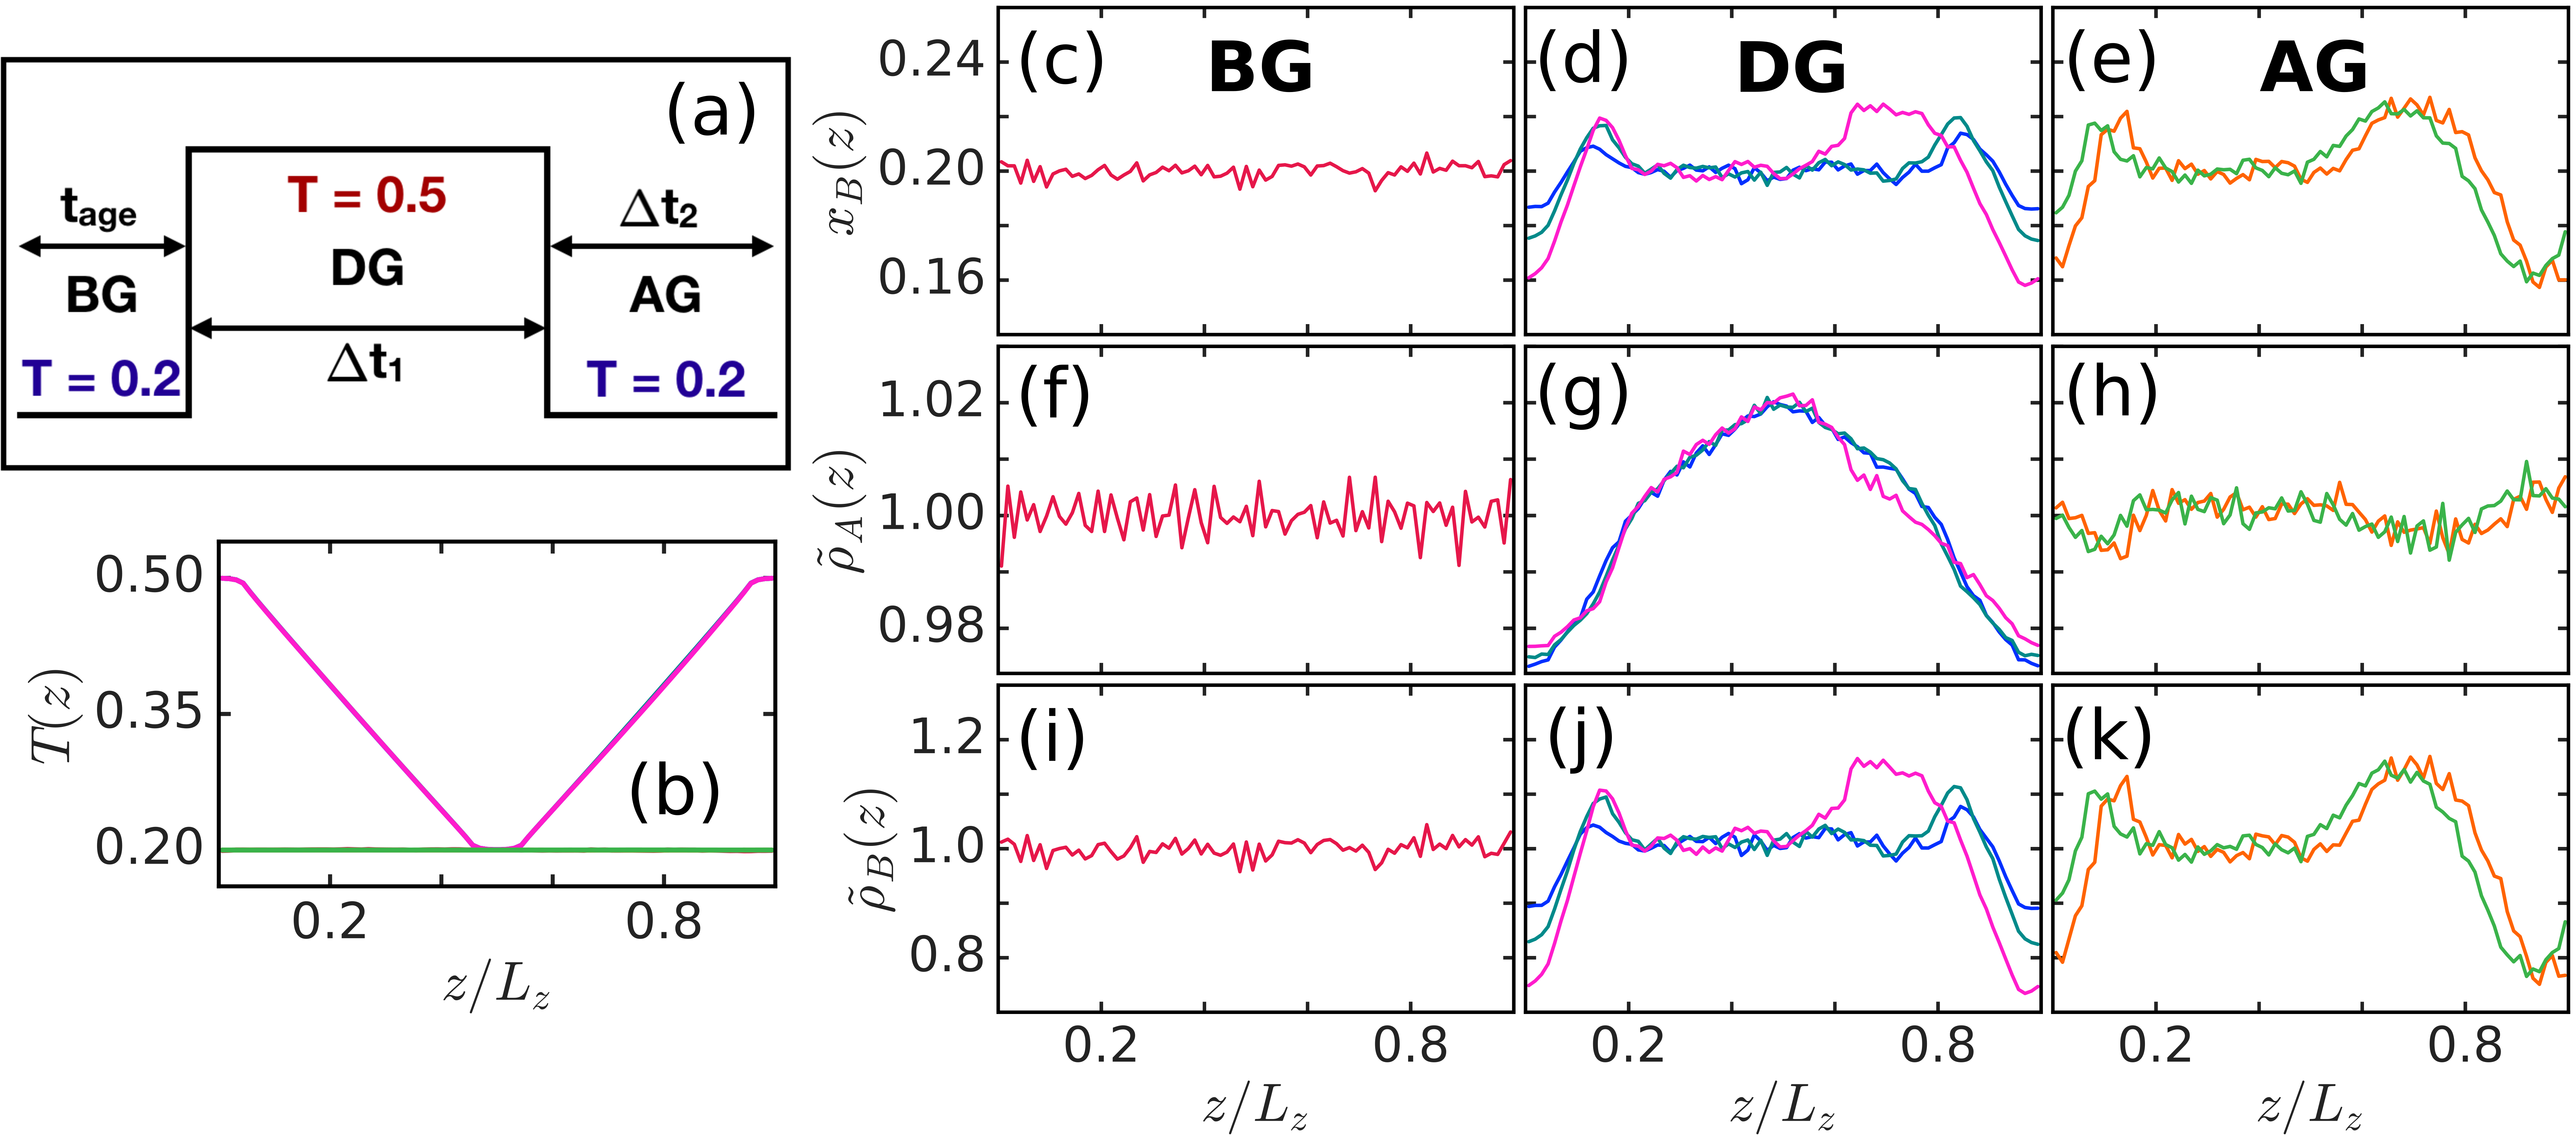
\includegraphics[scale=0.45]{figs/fig3p11.png}}
	\caption[{\em Response to a thermal gradient {\em pulse} with $T_{\rm h}=0.5$ and $T_{\rm c}=0.2$}]{Response to a thermal gradient {\em pulse} with $T_{\rm h}=0.5$ and $T_{\rm c}=0.2$. (a) Schematic of the protocol (see text).  (b) Spatial temperature profile during the protocol.  (Panels below) Time evolution of the spatial profiles, during BG, DG, AG [from left to right] (c)-(e) for concentration of B particles, (f)-(h) density of A particles, (i)-(k) density of B particles.  In (d), (g), (j), the curves are shown for $\Delta{t}/10^4=0-5$(blue), $5-10$(cyan), $45-50$(magenta).  Similarly, in (e), (h), (k), the curves are shown for $\Delta{t}/10^4=4-5$(orange), $49-50$(green).
	\label{fig3p11}}
\end{figure}
%

\section{Conclusions} 

We have studied the response of a glass-forming LJ mixture to an applied thermal gradient, in order to explore the interplay of heat transport and interdiffusive processes, as the mean ambient temperature is lowered from the supercooled regime towards the glass transition. Unlike the fast heat transport, structural relaxations and consequently interdiffusion exhibit a drastic slowing-down with decreasing temperature. In combination with chemical ordering effects, this results in increased concentration gradients and thereby larger Soret coefficients.  Due to the divergence of structural relaxation time scales, such features get suppressed in the glass. Moreover, the linear coupling between heat transport and interdiffusion breaks down when the thermal gradient is large, and the lower bound for this breakdown decreases while approaching the glassy regime. We note here that various studies have pointed out the observation of a significant finite-size effect in related systems (e.g. \cite{chantrenne2004finite, simonnin2017diffusion}), particularly in the measurement of transport coefficients; so, a systematic finite-size study of the transport behaviour explored in this work should be performed in future.

By applying a thermal gradient which leads to local melting of the glass, and then switching it off, we also demonstrate that it is possible to freeze in {concentration inhomogeneities} in a glass.  Such a protocol thus provides a possible route to design amorphous solids with specific concentration profiles.  

More such time-dependent protocols need further exploration to achieve needed functionalities, as well as to understand current practices in different applications, e.g.~laser-induced melting/welding. Similarly, controlled experiments using simple glass-formers are also necessary to support such computational studies.  {A recent study using X-ray radiography of an Al-Ni mixture \cite{sondermann2019} has demonstrated that it is possible to obtain  accurate experimental values of the Soret coefficient for real systems with similar properties as the LJ model, considered in this work.} On the theoretical side of understanding such phenomena, limited explorations have occurred from a microscopic perspective, especially in the approach to glass transition, and our work aims at motivating further studies in this direction.